%%==============================================================
%% Autor: Matheus dos Reis de Jesus
%% Última versão Maio/2021
%% Arquivo em formato UTF-8
%% Compilar com pdftex
%% Precisa do arquivo abntex2-UFV.sty e abntex2cite.tex
%%
%% Modelo: Rodrigo Smarzaro (smarzaro@ufv.br)
%%==============================================================

\documentclass[
	% -- opções da classe memoir --
	12pt,				    % tamanho da fonte
	openright,			    % capítulos começam em pág ímpar (insere página vazia caso preciso)
	oneside,			    % para impressão só no anverso. Oposto a twoside
	a4paper,			    % tamanho do papel.
    % -- opções do pacote abntex2 --
    % chapter=TITLE,         % Títulos em maiúsculas
    sumario=tradicional,    % Sumário padrão memoir (mais bonito "imo")
    % -- opções do pacote babel --
	english,			    % idioma adicional para hifenização
	brazil,				    % o último idioma é o principal do documento
	]{abntex2}              % Personaliza a capa. Precisa do arquivo ufv.cls para funcionar.


% Pacotes fundamentais
\usepackage{abntex2-UFV}        % Personalização para a Universidade Federal de Viçosa
\usepackage{lmodern}			% Usa a fonte Latin Modern			
\usepackage[T1]{fontenc}		% Selecao de codigos de fonte de saída
\usepackage[utf8]{inputenc}		% Codificacao do documento (conversão automática dos acentos)
\usepackage{indentfirst}		% Indenta o primeiro parágrafo de cada seção.
\usepackage{graphicx}			% Inclusão de gráficos
\usepackage{float}				% Posicionamento específico de figuras
\usepackage{booktabs}           % \toprule, \midrule e \bottomrule para tabelas
\usepackage{hyperref}
\usepackage{csquotes}
\usepackage{listings}			% Para trechos de código
\usepackage{subfig}
% Sistema autor-data com títulos nas referências em negrito
% \usepackage[abbrv,abnt-emphasize=bf]{abntex2cite}
\usepackage[backend=biber, style=numeric]{biblatex}
\addbibresource{referencias.bib}

% ---
% CONFIGURAÇÕES DE PACOTES
% ---

% Informações de dados para CAPA e FOLHA DE ROSTO
\titulo{\emph{Desenvolvimento de um UI Framework em React Native com componentes focados em acessibilidade para idosos em dispositivos móveis}}
\autor{Matheus dos Reis de Jesus}
\local{Viçosa}
\data{2021}
\orientador{Lucas Francisco da Matta Vegi}    % redefinido no abntex2-UFV para aceitar Instituição (default = UFV-CRP)
%\coorientador{Nome do Coorientador}
\instituicao{Universidade Federal de Viçosa}

\campus{\emph{Campus} de Viçosa}      % pacote abntex2-UFV
\curso{Ciência da Computação}               % pacote abntex2-UFV
%\membrobancaA{Membro da Banca A}             % pacote abntex2-UFV default = UFV-CRP
%\membrobancaB[UFMG]{Membro da Banca B}       % pacote abntex2-UFV default = UFV-CRP
%\databanca{\today}                           % pacote abntex2-UFV

% O preambulo deve conter o tipo do trabalho, o objetivo,
% o nome da instituição e a área de concentração
\preambulo{Projeto apresentado à Universidade Federal de Viçosa como parte das exigências para a aprovação na disciplina Seminários II}
% ---

% ---
% Configurações de aparência do PDF final

% informações para o arquivo pdf de saída
% Interessante alterar a cor dos links para preto(black)
% para imprimir
\makeatletter
\hypersetup{
        % metadados
		pdftitle={\@title},
		pdfauthor={\@author},
    	pdfsubject={\imprimirpreambulo},
	    pdfcreator={LaTeX with abnTeX2},
		colorlinks=true,   % false: links em frame; true: links coloridos
    	linkcolor=black,    % cor dos links no documento
    	citecolor=blue,    % cor dos links para a bibliografia
    	filecolor=magenta, % cor dos links para arquivos
		urlcolor=blue,     % cor dos links para sites
		bookmarksdepth=4   % profundidade do sumário do PDF
}
\makeatother
% ---

\begin{document}
% Retira espaço extra obsoleto entre as frases.
\frenchspacing

% ----------------------------------------------------------
% ELEMENTOS PRÉ-TEXTUAIS
% ----------------------------------------------------------
\pretextual

% Capa
\imprimircapa

% Folha de rosto
\imprimirfolhaderosto
% ---

% Inserir folha de aprovação
%\imprimirfolhadeaprovacao

% Dedicatória
%\begin{dedicatoria}
%   \vspace*{\fill}
%   \centering
%   \noindent
%   \textit{Texto qualquer da dedicatória}
%   \vspace*{\fill}
%\end{dedicatoria}
% ---

% Agradecimentos
%\begin{agradecimentos}

%\end{agradecimentos}
% ---

% Epígrafe
%\begin{epigrafe}
%    \vspace*{\fill}
%	\begin{flushright}
%		\textit{``Word? nunca mais.''\\
%		(Qualquer usuário de \LaTeX)}
%	\end{flushright}
%\end{epigrafe}
% ---

% RESUMOS

% resumo em português
\begin{resumo}
	\noindent

	\MakeUppercase{\textbf{Desenvolvimento de um UI Framework em React Native com componentes focados em acessibilidade para idosos em dispositivos móveis}}

	\vspace{\onelineskip}
	Lucas Francisco da Matta Vegi (Orientador) \newline
	Matheus dos Reis de Jesus (Estudante)
	\vspace{\onelineskip}

	\MakeUppercase{\textbf{Resumo}}

	A constante evolução da tecnologia tem trazido cada vez mais recursos inovadores que têm transformado a maneira como interagimos com o mundo. De um computador de mesa à um dispositivo móvel, a quantidade de recursos que temos à nossa disposição é quase imensurável. Porém, esses recursos têm suas limitações, principalmente por alcançarem públicos diversos e não necessariamente estarem preparados para lidar com as necessidades que estes possuem. Especialmente em dispositivos móveis, grande parte das aplicações não possuem recursos que possibilitem o uso por pessoas com necessidades especiais, como por exemplo pessoas idosas. Tendo isso em mente, este trabalho desenvolveu componentes que podem ser reutilizados durante o desenvolvimento de aplicativos móveis que terão idosos como usuários. Esses componentes são compatíveis com todos os principais sistemas operacionais modernos para dispositivos móveis e permitem que as principais dificuldades enfrentadas por idosos ao tentar utilizar estes dispositivos sejam contornadas.

	\vspace{\onelineskip}

	\noindent
	\MakeUppercase{\textbf{Palavras-chaves}} \newline
	Acessibilidade, React Native, Framework, UI
	\vspace{\onelineskip}

	\noindent
	\MakeUppercase{\textbf{Área de Conhecimento}} \newline
	1.03.03.04-9 Sistemas de Informação
	\vspace{\onelineskip}

	\noindent
	\MakeUppercase{\textbf{Linha de Pesquisa}} \newline
	DPI-016 – Sistemas de Informação
\end{resumo}

% resumo em inglês
%\begin{resumo}[Abstract]
% \begin{otherlanguage*}{english}
%   \noindent
%   % Insira o abstract aqui
%
%   \vspace{\onelineskip}
%
%   \noindent
%   \textbf{Key-words}: TCC, latex, abntex, UFV..
% \end{otherlanguage*}
%\end{resumo}

% inserir lista de ilustrações
\pdfbookmark[0]{\listfigurename}{lof}
\listoffigures*
\cleardoublepage
% ---

% inserir lista de tabelas
\pdfbookmark[0]{\listtablename}{lot}
\listoftables*
\cleardoublepage
% ---


% inserir o sumario
\pdfbookmark[0]{\contentsname}{toc}
\tableofcontents*
\cleardoublepage
% ---

% ----------------------------------------------------------
% ELEMENTOS TEXTUAIS
% ----------------------------------------------------------
\textual

\chapter{Introdução}\label{sec:introducao}

Segundo a \emph{30ª Pesquisa Anual de Uso de TI},
realizada pela \emph{Fundação Getúlio Vargas}\cite{pesquisati30}, em abril de 2019 o Brasil já contava com aproximadamente 230 milhões de dispositivos móveis, pouco mais de 1 dispositivo móvel por habitante. Já na 31ª edição\cite{pesquisati31}, de junho de 2020, esse valor passou para de 342 milhões de dispositivos móveis, equivalente a aproximadamente 1,6 dispositivos por habitante. De acordo com dados do sensos realizados pelo IBGE, a população idosa(pessoas adultas acima de 65 anos) no Brasil cresceu de 8.9 milhões em 2017 para 9.8 milhões em 2020, um aumento de aproximadamente 11\% em 3 anos\cite{ibge}.

\par

Com o crescimento vertiginoso do uso de dispositivos móveis, há um aumento da demanda por aplicações que possam atender às mais diversas necessidades das pessoas que os utilizam. Levando em consideração os dados citados previamente, é plausível considerar que boa parte dos novos dispositivos pertençam à pessoas da terceira idade, que comumente apresentam dificuldade para executar diversas ações que são essenciais na interação de dispositivos móveis, em especial, os com tela tátil. Além dos fatores mais comuns, pessoas idosas apresentam problemas motores, de visão e cognitivos, que tornam ainda mais difíceis essas interações. Segundo Claudia Zapata \emph{et al}, “O desenvolvimento de aplicações para dispositivo móveis se tornou uma forma de melhorar a qualidade de vida para idosos, já que é possível aplicar a vários setores como a medicina, por exemplo”\cite{elderlyMainChallenges}.

\section{Objetivo}\label{sec:objetivos}

\subsection{Geral}

A proposta deste trabalho é implementar o \emph{ElderlyFrame} utilizando \emph{React Native}, uma tecnologia para desenvolvimento multiplataforma para dispositivos móveis, visando ampliar o impacto do mesmo e criar novas possibilidades de uso da ferramenta.

\subsection{Específicos}

Como objetivos específicos, propunha-se:

\begin{itemize}
	\item Analisar do \textit{ElderlyFrame} para embasamento
	\item Desenvolver o novo \textit{framework} utilizando uma tecnologia multiplataforma
	\item Desenvolver uma aplicação para teste dos componentes do \textit{framework}
	\item Ter como resultado final uma ferramenta reutilizável e facilitadora das interações de pessoas idosas com dispositivos móveis
\end{itemize}

\chapter{Referencial Teórico}\label{sec:referencialTeorico}

\section{ElderlyFrame}

Em uma conversa com o orientador deste projeto, Lucas Vegi, conheci a tese de mestrado desenvolvida pela Dâmaris Arruda: Um \textit{framework} para facilitar as interações entre dispositivos móveis e pessoas idosas\cite{tesedamaris}.

\par

Em sua tese, Dâmaris buscou identificar as ações em dispositivos móveis que os idosos enfrentam maior dificuldade para executar. Para conseguir identificar algumas dessas dificuldades, foram realizados testes em um trabalho conjunto com o \emph{Programa da Terceira Idade}, um projeto da Prefeitura Municipal de Viçosa - MG. Através destes testes foram identificadas algumas das ações que os idosos mais apresentam dificuldade em executar: o movimento de pinça, movimento de rotação e digitação.

\par

Com o resultado das pesquisas em mãos, foi então criado o \textit{ElderlyFrame}\cite{elderlyframe}, um \textit{framework} de interface de usuário nativo para \textit{Android}. O projeto contém um conjunto de componentes visuais com o objetivo de facilitar ações que geralmente exigem mais coordenação motora e acuidade visual. A seguir, temos os exemplos destes componentes que foram implementados.

\begin{figure}[H]
	\begin{center}
		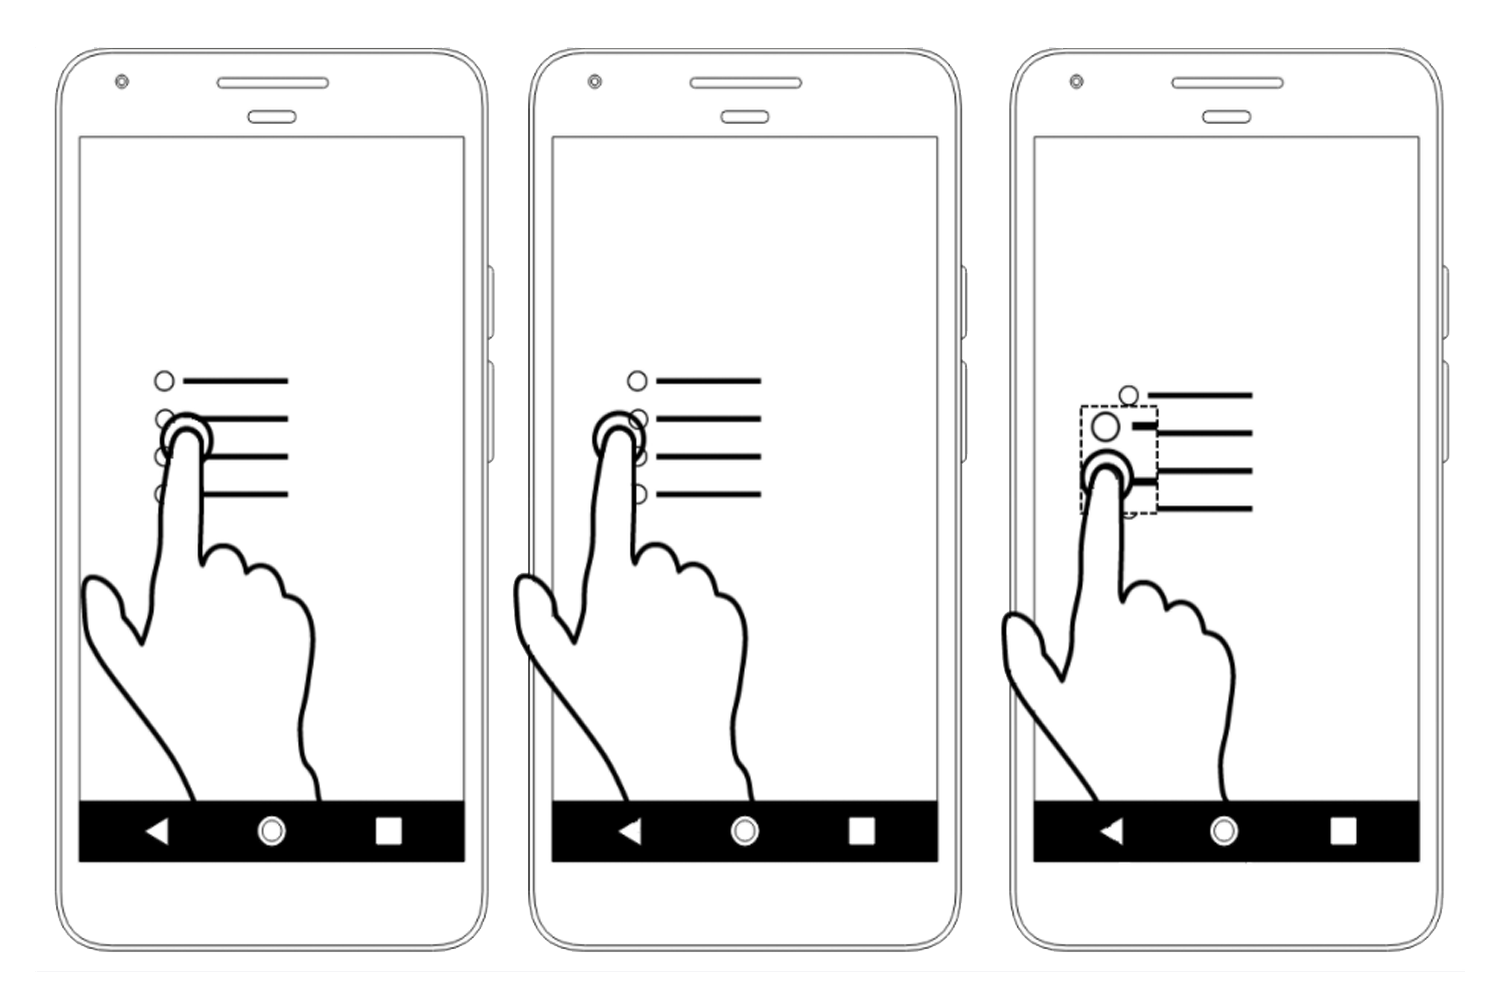
\includegraphics[height=0.4\linewidth]{images/touchable-zoom.png}
	\end{center}
	\caption[Componente \textit{TouchZoom} do \textit{ElderlyFrame}]{Componente de Zoom por toque do \textit{ElderlyFrame}}
	\legend{Fonte: \citeauthor{tesedamaris} \cite{tesedamaris}}
	\label{fig:touchableZoom}
\end{figure}

\begin{figure}[H]
	\begin{center}
		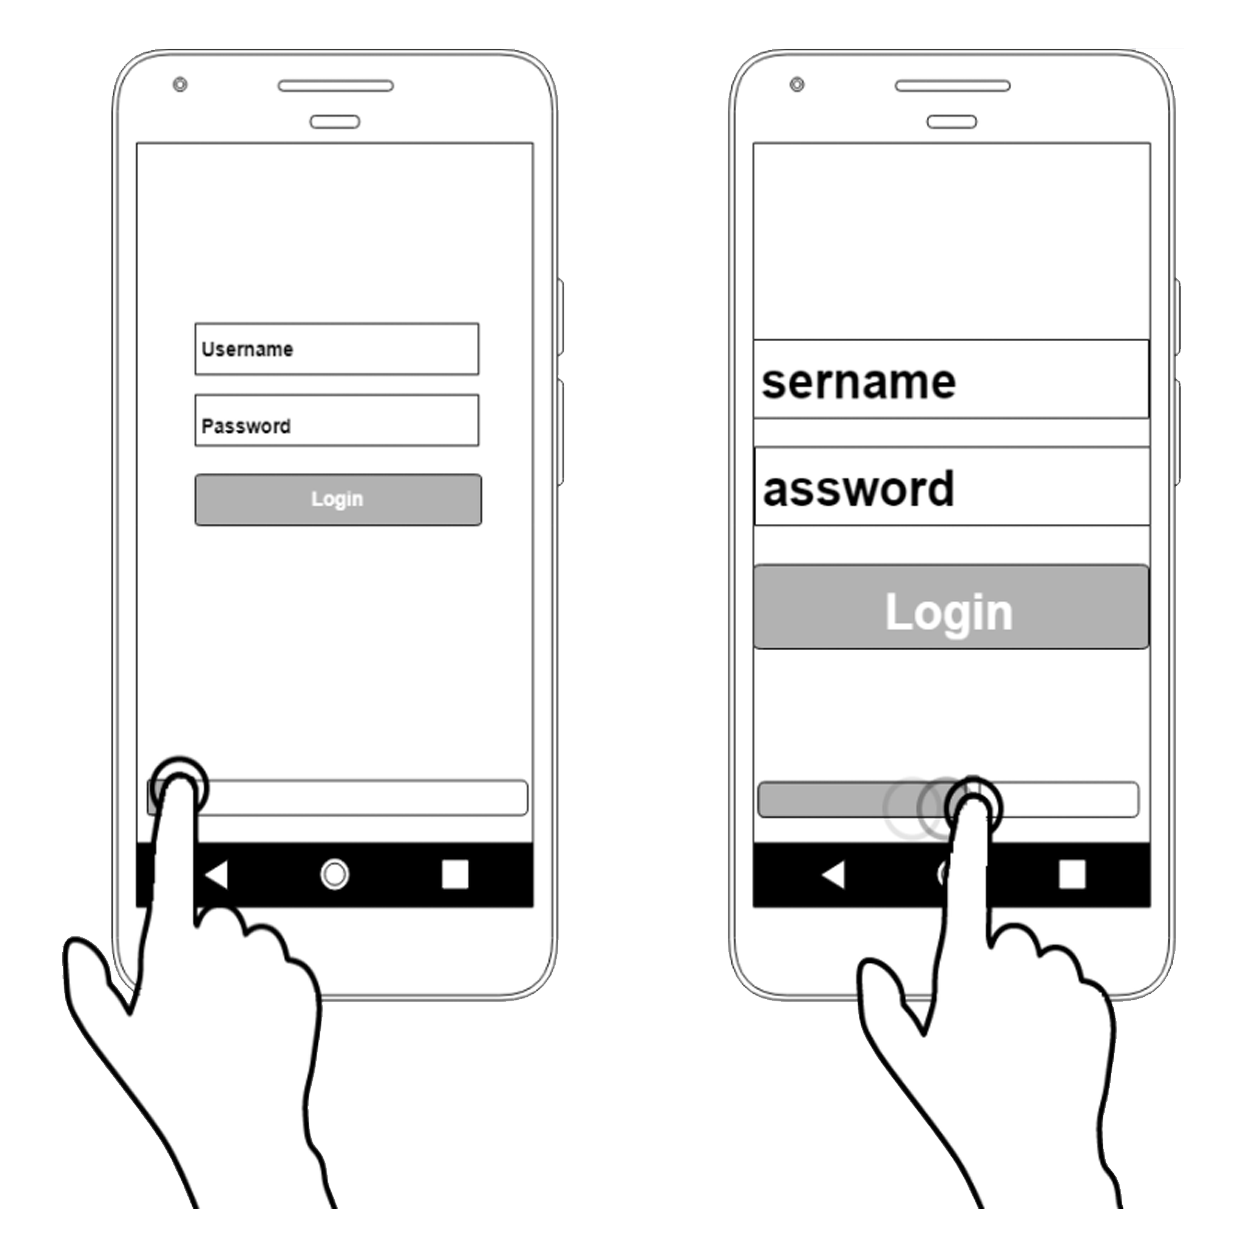
\includegraphics[height=0.5\linewidth]{images/zoom-bar.png}
	\end{center}
	\caption[Componente \textit{SeekBarZoom} do \textit{ElderlyFrame}]{Componente de Zoom por barra do \textit{ElderlyFrame}}
	\legend{Fonte: \citeauthor{tesedamaris} \cite{tesedamaris}}
	\label{fig:zoomBar}
\end{figure}

\begin{figure}[H]
	\begin{center}
		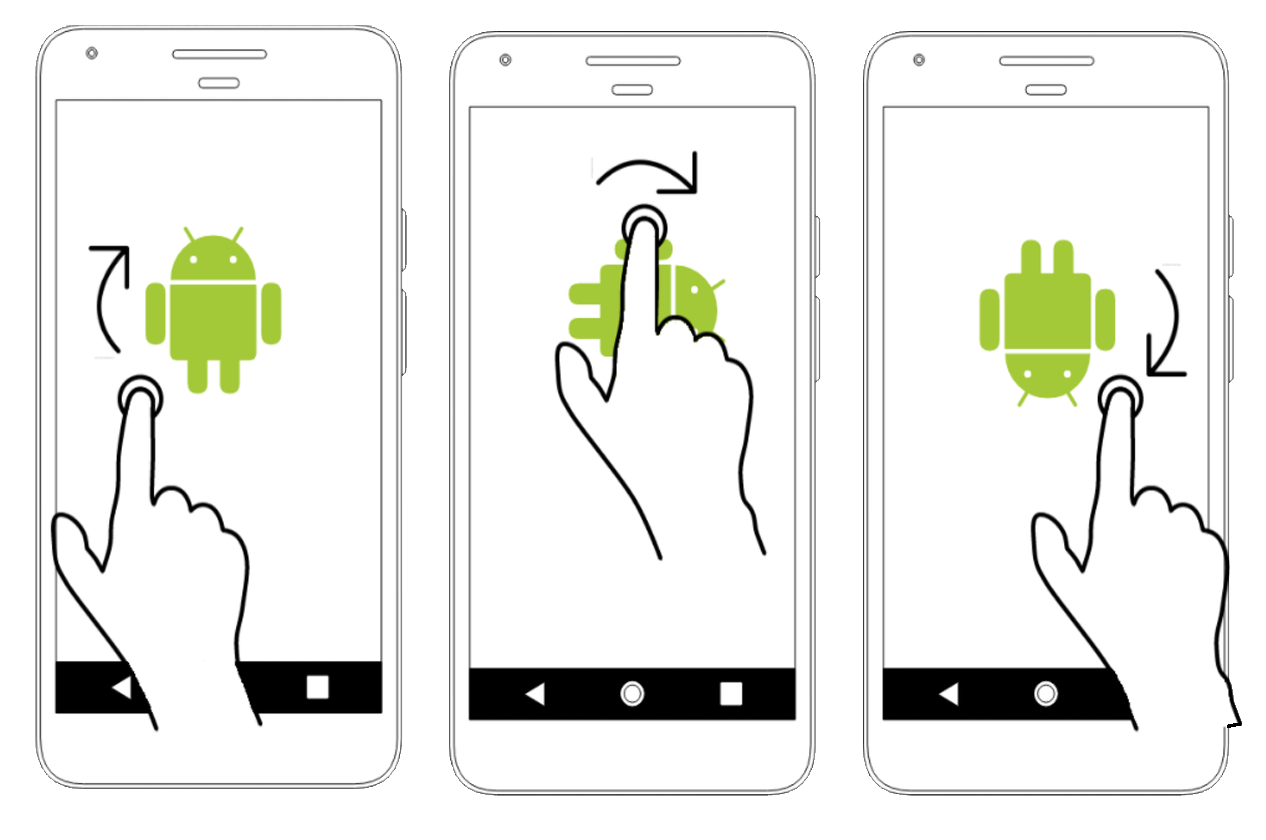
\includegraphics[height=0.5\linewidth]{images/rotation.png}
	\end{center}
	\caption[Componente \textit{SimpleRotation} do \textit{ElderlyFrame}]{Componente de rotação com apenas um dedo do \textit{ElderlyFrame}}
	\legend{Fonte: \citeauthor{tesedamaris} \cite{tesedamaris}}
	\label{fig:rotation}
\end{figure}

\begin{figure}[H]
	\begin{center}
		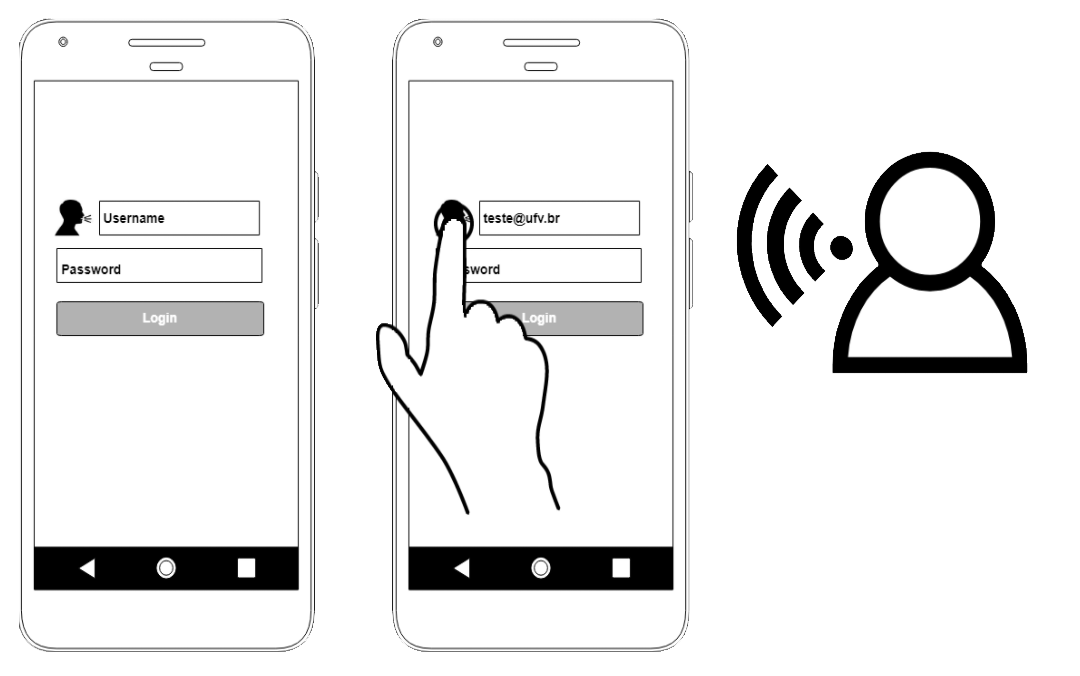
\includegraphics[height=0.5\linewidth]{images/speech-to-text.png}
	\end{center}
	\caption[Componente \textit{SpeechToText} do \textit{ElderlyFrame}]{Componente de conversão de voz para texto (\textit{speech-to-text}) do \textit{ElderlyFrame}}
	\legend{Fonte: \citeauthor{tesedamaris} \cite{tesedamaris}}
	\label{fig:speechToText}
\end{figure}

\section{Desenvolvimento multiplataforma}

Como dito anteriormente, o \textit{ElderlyFrame} é um \textit{framework} de interface de usuário nativo para \textit{Android}, e este é um fator limitante da sua utilização. Ampliar o impacto do projeto e abranger uma maior parcela do cenário de desenvolvimento para dispositivos móveis são fatores motivadores para este projeto. Para isto, decidiu-se por focar em uma tecnologia de desenvolvimento multiplataforma. Tecnologias de desenvolvimento multiplataforma permitem o desenvolvimento de aplicações para diferentes sistemas operacionais, como \emph{Android} e \emph{iOS}, utilizando uma mesma base de código.

\begin{figure}[H]
	\begin{center}
		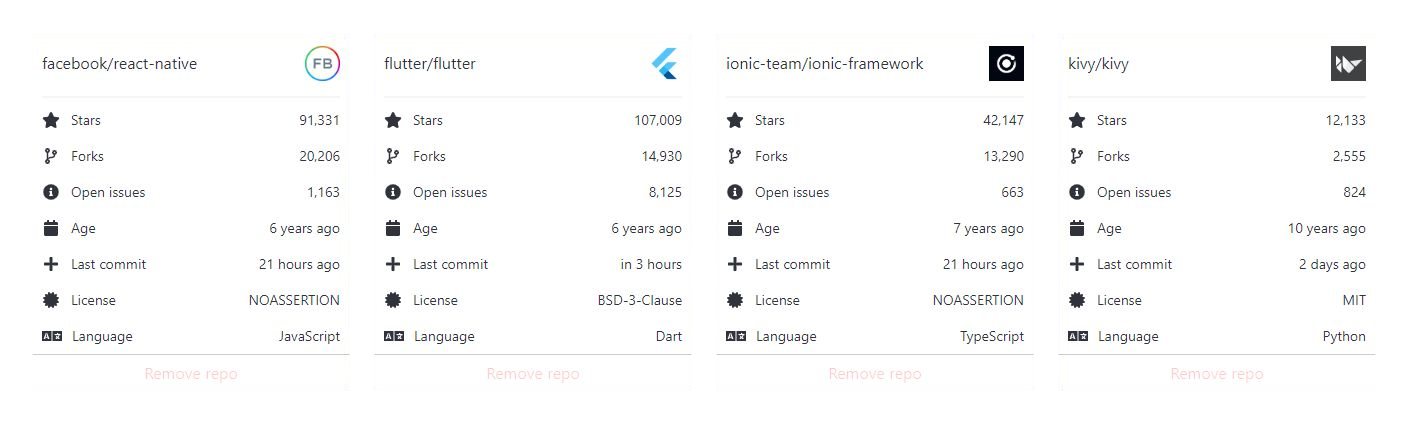
\includegraphics[width=1\linewidth]{images/github-compare.png}
	\end{center}
	\caption[Comparativo de estatísticas dos repositórios de tecnologias de desenvolvimento multiplataforma]{Comparação entre as estatísticas dos repositórios de tecnologias de desenvolvimento multiplataforma: \textit{React Native}, \textit{Flutter}, \textit{Ionic} e \textit{Kivy}}
	\label{fig:githubCompare}
	\legend{Fonte: \textit{GitHub Compare}. Disponível em \url{https://www.githubcompare.com/facebook/react-native+flutter/flutter+ionic-team/ionic-framework+kivy/kivy/}}
\end{figure}

A imagem acima mostra que o repositório do \textit{React Native}, no \textit{GitHub}, tem a maior quantidade de \textit{forks} e o 2º maior número de \textit{stars} e \textit{issues}, quando comparado com outras tecnologias de desenvolvimento multiplataforma, a saber: \textit{Flutter},\textit{Ionic} e \textit{Kivy}.

Além das estatísticas apresentadas no parágrafo anterior, foi usada como uma base uma pesquisa realizada pela \textit{Statista}, que aborda o uso de \textit{frameworks} para desenvolvimento multiplataforma. Como pode ser observado, o \textit{React Native} representa aproximadamente 42\% do uso em aplicações.

\begin{figure}[H]
	\begin{center}
		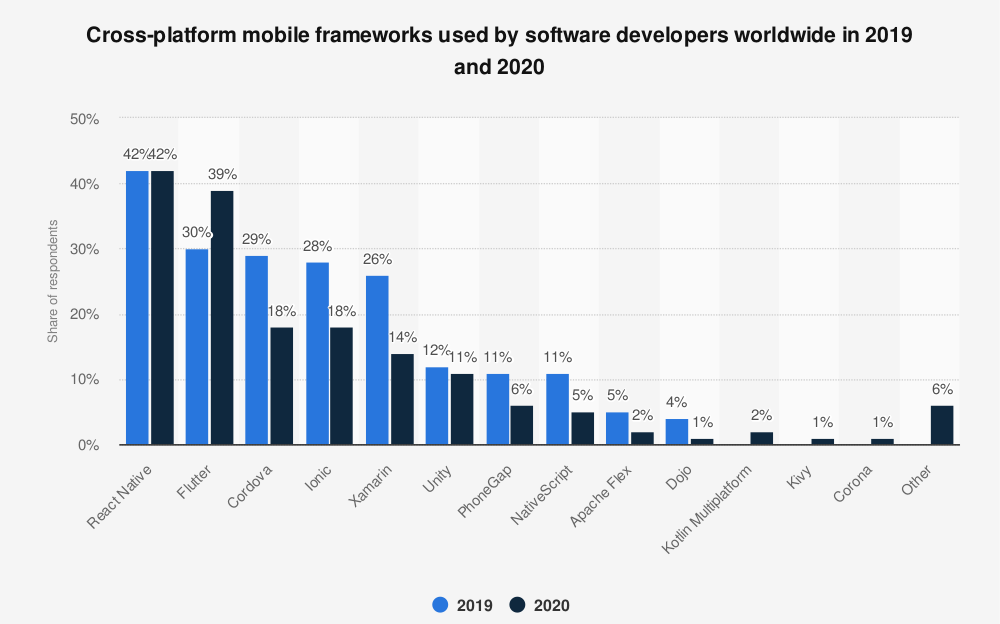
\includegraphics[height=.5\linewidth]{images/mobile-frameworks-statista.png}
	\end{center}
	\caption[Comparativo de uso de frameworks para desenvolvimento multiplataforma]{Comparação entre as estatísticas de uso de \textit{frameworks} para desenvolvimento multiplataforma}
	\label{fig:statistaResearch}
	\legend{Fonte: \citeauthor{statista} \cite{statista}}
\end{figure}

Em um cenário com tantas opções, a tecnologia \textit{React Native} se destaca sobre as demais, e inclusive é utilizado em aplicações com grande representatividade, como \textit{Instagram}, \textit{AirBnb} e \textit{Uber}.

\section{Trabalhos prévios}

Atualmente existem implementações para \textit{React Native} de ferramentas que facilitam a presença de recursos de acessibilidade em aplicações para dispositivos móveis. Porém, estas ferramentas utilizam apenas recursos já existentes, como, por exemplo, para mecanismo de leitura de tela, funcionando apenas como facilitadoras. Este é um diferencial do \textit{ElderlyFrame}, e consequentemente deste projeto, que traz uma nova abordagem para interações que pessoas idosas apresentam dificuldade em executar.

\par

Em pesquisas realizadas para elaboração deste projeto, somente foram encontrados artigos e teses que abordavam a teoria da acessibilidade para idosos, falta de inclusão digital da terceira idade, falta de recursos de acessibilidade em aplicações para dispositivos móveis e afins. Porém, foi notada uma carência de projetos que de fato produzissem algo para mudar este cenário. O \textit{ElderlyFrame} foi construído com este propósito, e essa é uma das motivações desta pesquisa.

\chapter{Metodologia}\label{sec:metodologia}

Para dar início a este trabalho, primeiro foi necessário compreender o funcionamento do \textit{ElderlyFrame}. Para tal, foi criada uma aplicação para testes, em que foram utilizados todos os componentes implementados pelo framework. Dessa forma, foi possível identificar o funcionamento esperado de cada um, para serem posteriormente implementados no \textit{react-native-accessibility-elderly}, nome dado ao artefato produzido ao fim produzido através deste trabalho.

\section{O \textit{ElderlyFrame}}

Ao analisar a implementação do \textit{ElderlyFrame}, foi possível identificar alguns problemas. Como o foco principal do trabalho da Dâmaris foi a realização da pesquisa, imagino que isso possa ter impactado o resultado final da implementação.

Como a primeira versão do \textit{ElderlyFrame} foi publicada em 2019, 2 anos antes do desenvolvimento deste presente trabalho, fez-se necessário realizar algumas mudanças, pois as tecnologias usadas passaram por atualizações e melhorias, fazendo com que tais alterações fossem necessárias. Abaixo temos uma lista do que foi modificado:

\begin{itemize}
	\item Atualização da ferramenta \textit{gradle} para a versão 5.1.1
	\item Atualização da \textit{minSdkVersion} para a versão 16
	\item Atualização da \textit{compileSdkVersion} para a versão 30
	\item Mudança repositório central de \textit{JCenter} para \textit{MavenCentral}
	\item Mudança do pacote \textit{android.support} para o pacote \textit{androidx}
	\item Correção na implementação do ícone do componente \textit{SpeechText}
\end{itemize}

Para fins de registro das modificações realizadas, foi feito um \textit{fork} do projeto da \textit{ElderlyFrame} na plataforma \textit{GitHub}, que pode ser acessado no link abaixo: \linebreak

\href{https://github.com/reisdev/elderlyframe/}{https://github.com/reisdev/elderlyframe}.


\section{O framework \textit{react-native-accessibility-elderly}}

\par

A ideia inicial era implementar o framework de forma nativa. Ou seja, os trechos de código seriam escritos separadamente para cada plataforma. Para \textit{iOS}, usando \textit{Swift} ou \textit{Objective-C}, e para \textit{Android}, usando \textit{Java} ou \textit{Kotlin}. Porém, a tecnologia utilizada, \textit{React Native}, ainda apresenta algumas limitações com relação à implementação de módulos nativos, e isso levou à decisão de criar os componentes utilizando apenas \textit{Javascript} e \textit{Typescript}, linguagens usadas pela própria tecnologia.

\subsection{Recursos de terceiros}

A criação dos componentes do framework exigiu que algumas bibliotecas de terceiros fossem utilizadas, pois as mesmas forneciam recursos que demandariam muito esforço para serem implementados, que não caberia dentro dos prazos do projeto. Abaixo, temos a especificação de cada biblioteca e os recursos que as mesmas oferecem:

\begin{itemize}
	\item \textit{@react-native-voice/voice}: Reconhecimento de voz e conversão de voz para texto
	\item \textit{@react-native-community/slider}: Componente \textit{Slider} para \textit{React Native}
	\item \textit{react-native-vector-icons}: Conjunto de ícones variados
	\item \textit{react-native-gesture-handler}: Reconhecimento de gestos na tela de um dispositivo móvel.
\end{itemize}

\subsection{Os desafios}

Uma das maiores barreiras encontradas ao desenvolver este framework foi o próprio \textit{React Native}. Apesar de ser uma tecnologia madura, ainda apresenta algumas limitações com relação ao desenvolvimento de pacotes.

\par

A ferramenta \textit{yarn}, alternativa ao \textit{npm}, foi usada para criar um ambiente de desenvolvimento, pois ela permite que uma aplicação e uma biblioteca sejam criadas num mesmo ambiente, compartilhando a instalação de pacotes e assim, reduzindo o espaço em disco necessário. Nesse sentido, o uso do \textit{yarn} foi essencial na hora de acelerar o processo de desenvolvimento e também de testes para validação do \textit{framework}.

\subsection{Publicação de pacote}

O \textit{react-native-accessibility-elderly} será um publicado em forma de pacote usando a ferramenta \textit{npm}, que é um gerenciador de pacotes. Sendo assim, qualquer pessoa que deseje criar uma aplicação para dispositivos móveis com recursos de acessibilidade para idosos, poderá utilizar os componentes deste framework através da instalação do pacote usando o \textit{npm}.

A tecnologia \textit{React Native} exige que pacotes com implementações nativas passem por um processo de \textit{link}, que consiste em referenciar as respectivas implementações para que as aplicações que as usam possam encontrar e utilizar seus recursos.

\chapter{Resultados}\label{sec:resultados}

\section{Código-fonte}

O código-fonte do \textit{framework} desenvolvido durante este trabalho foi criado em um repositório público, de código aberto, sob a liçença pública GNU v3.0. O repositório pode ser acessado através do link abaixo:

\href{https://github.com/reisdev/react-native-accessibility-elderly}{https://github.com/reisdev/react-native-accessibility-elderly}

\section{Componentes}

Todos os componentes contidos no \textit{EldelryFrame} foram devidamente implementados utilizando \textit{React Native}. A seguir, um detalhamento maior das especificidades de cada um e um exemplo de como utilizá-lo em uma aplicação para dispositivos móveis.

\subsection{Componente \textit{PinchZoom}}

O componente \textit{PinchZoom} implementa uma interação relativamente comum de se utilizar, que é a de pinça para aproximar um elemento. Sua implementação foi simples e inclusive foi possível aproveitar os conceitos aplicados no componente \textit{SeekBarZoom}, adaptados ao movimento de pinça. Abaixo, um exemplo de utilização do componente para desenvolvimento:

\begin{figure}[H]
	\begin{center}
		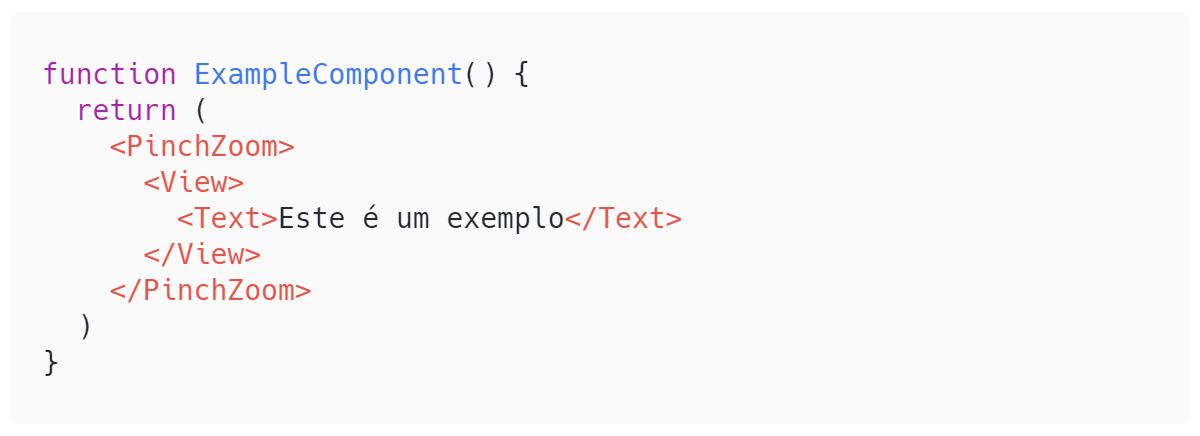
\includegraphics[width=.8\linewidth]{images/PinchZoom.png}
		\caption[Componente \textit{PinchZoom}]{Exemplo de utilização do componente \textit{PinchZoom}}
		\label{fig:pinchZoomExample}
		\legend{Fonte: Próprio Autor}
	\end{center}
\end{figure}

\par

A seguir, temos os exemplos da utilização do componente \textit{PinchZoom} em uma aplicação sendo executada nos sistemas operacionais \textit{iOS} e \textit{Android}

\begin{figure}[H]
	\centering
	\subfloat[Estado inicial do componente \textit{PinchZoom}]{
		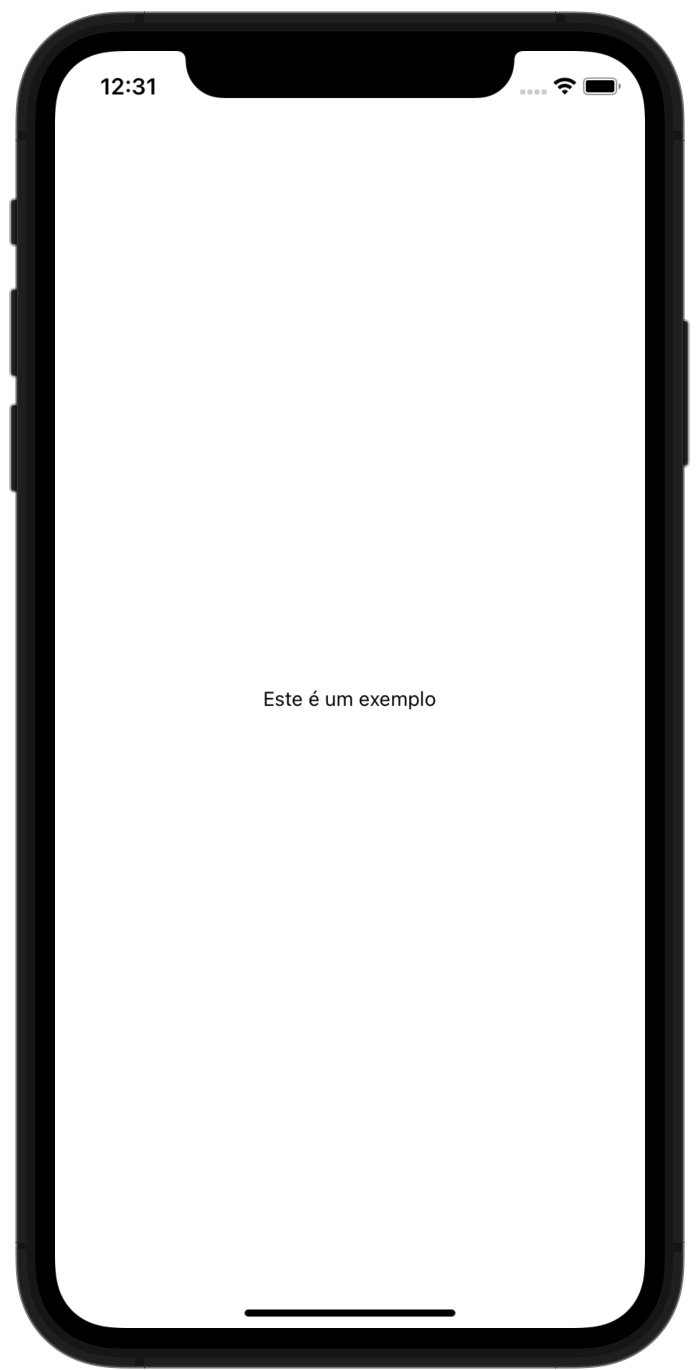
\includegraphics[width=.4\linewidth]{images/screenshots/iOS-PinchZoom-initial.png}}
	\hfill
	\subfloat[Estado do componente \textit{PinchZoom} após o movimento de pinça]{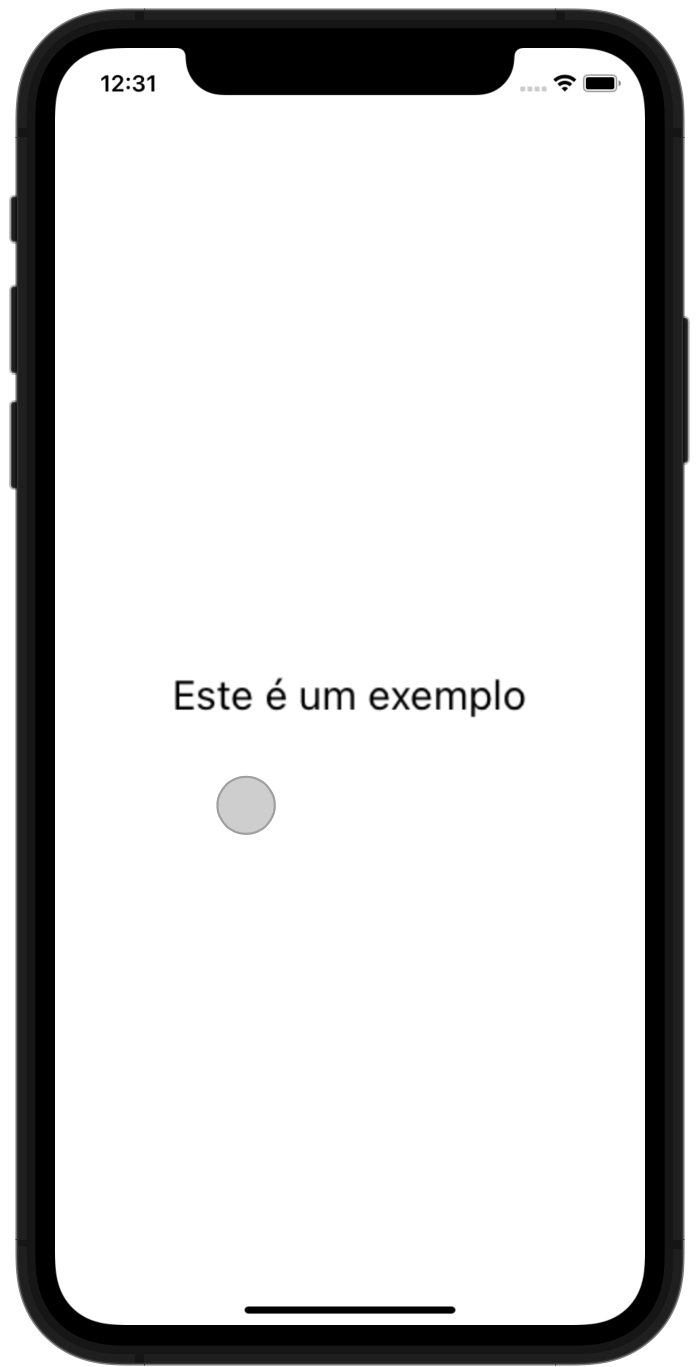
\includegraphics[width=.4\linewidth]{images/screenshots/iOS-PinchZoom-zoomed.png}}
	\caption[Componente \textit{PinchZoom} no \textit{iOS}]{Exemplo de utilização do componente \textit{PinchZoom} no \textit{iOS}}
	\label{fig:pinchZoomiOSExample}
	\legend{Fonte: Próprio Autor}
\end{figure}

\begin{figure}[H]
	\centering
	\subfloat[Estado inicial do componente \textit{PinchZoom}]{
		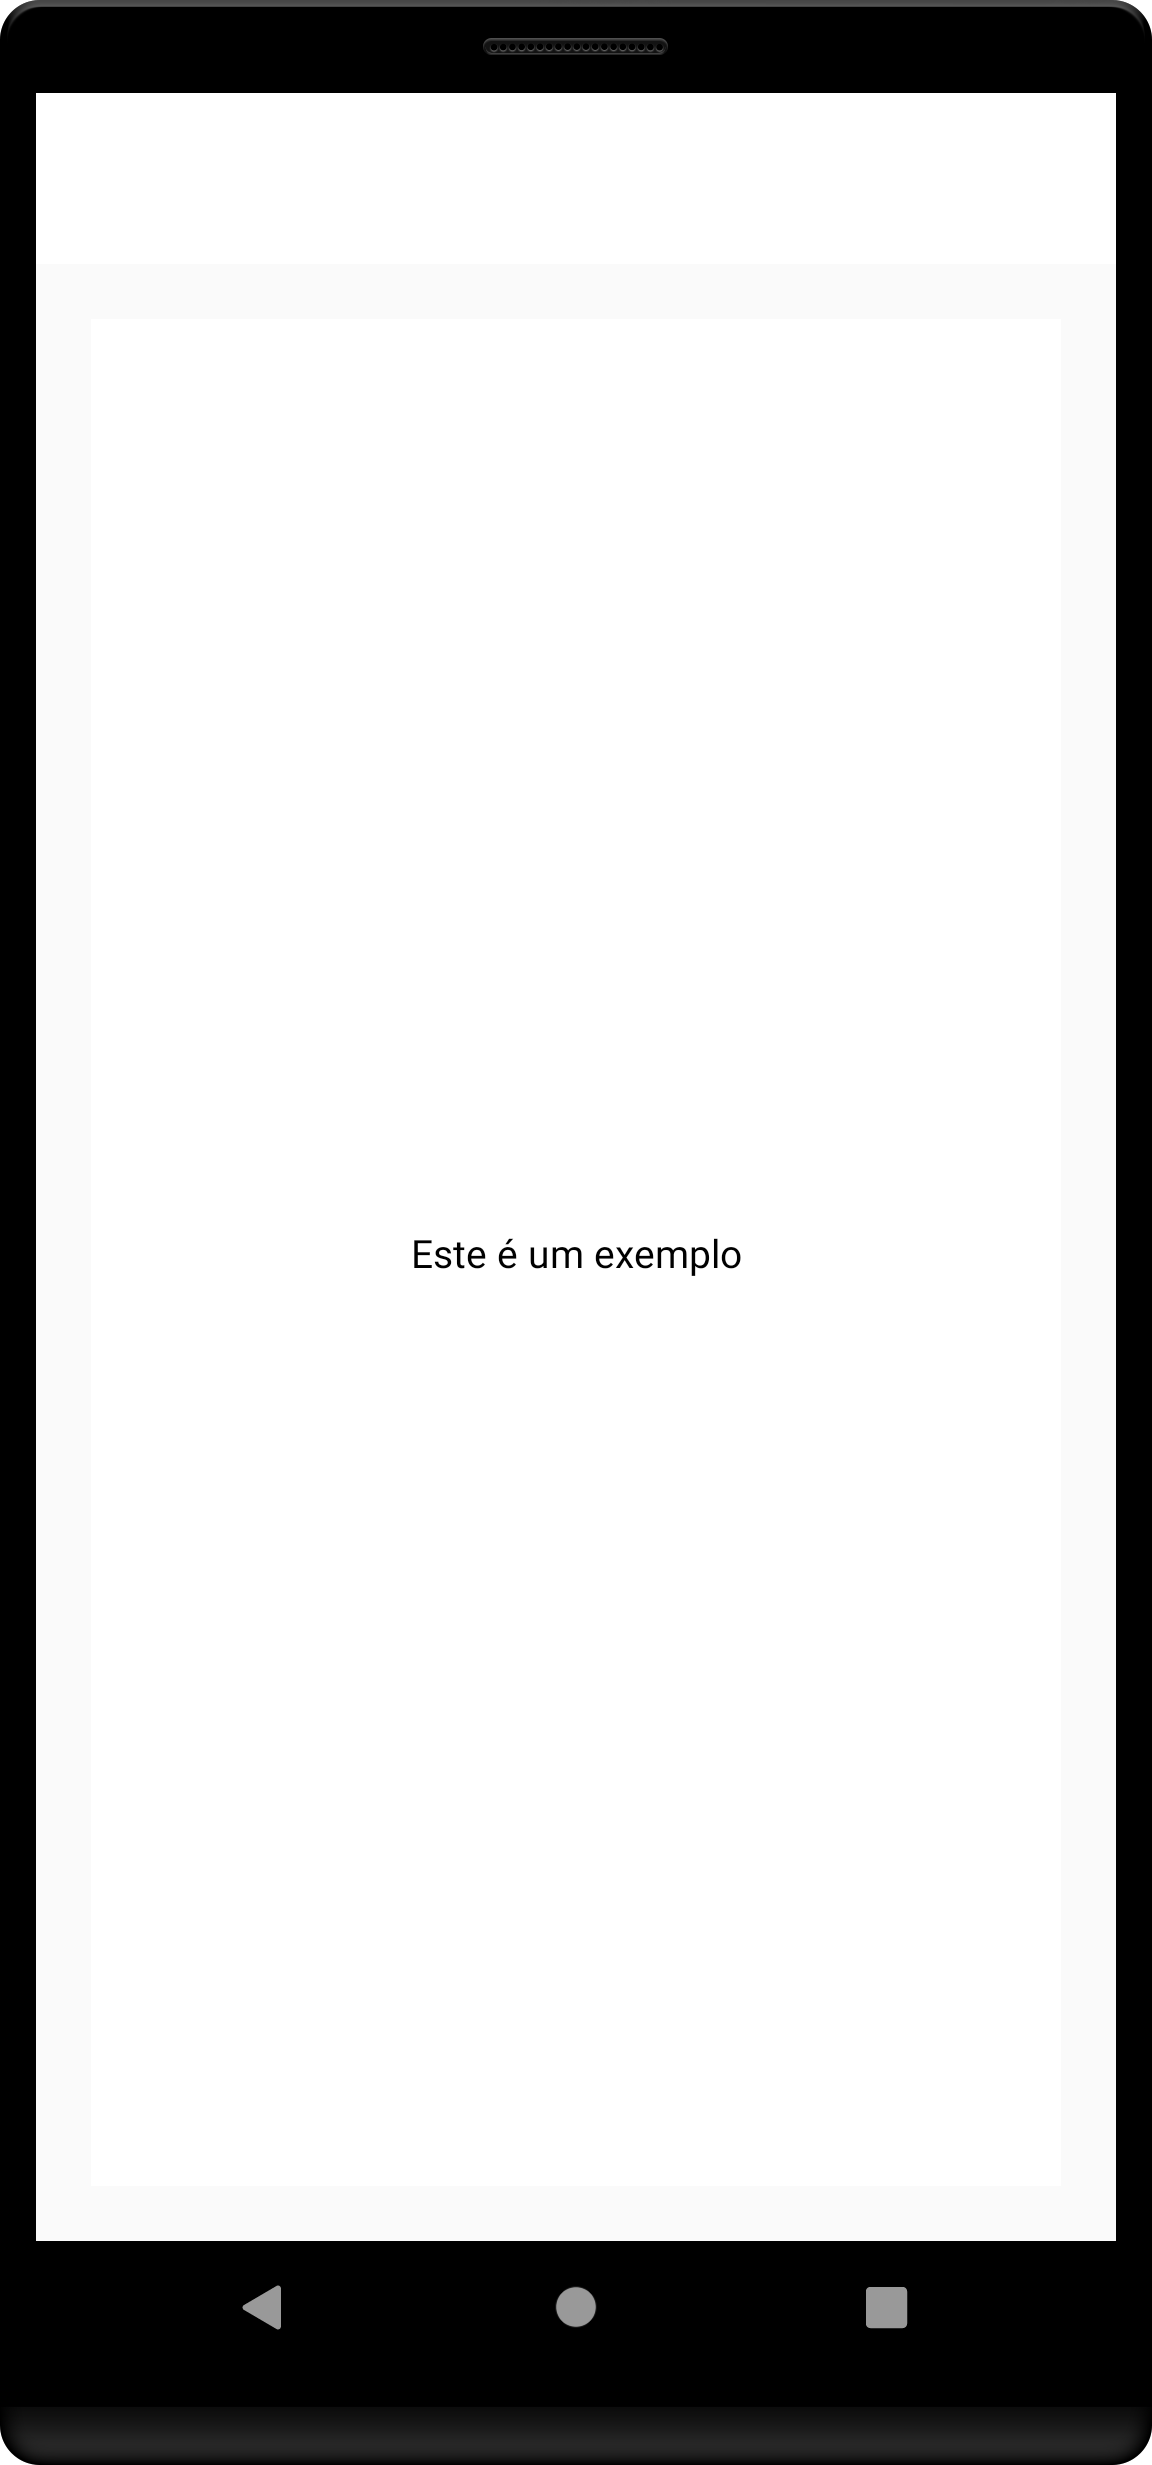
\includegraphics[width=.4\linewidth]{images/screenshots/Android-PinchZoom-initial.png}}
	\hfill
	\subfloat[Estado do componente \textit{PinchZoom} após o movimento de pinça]{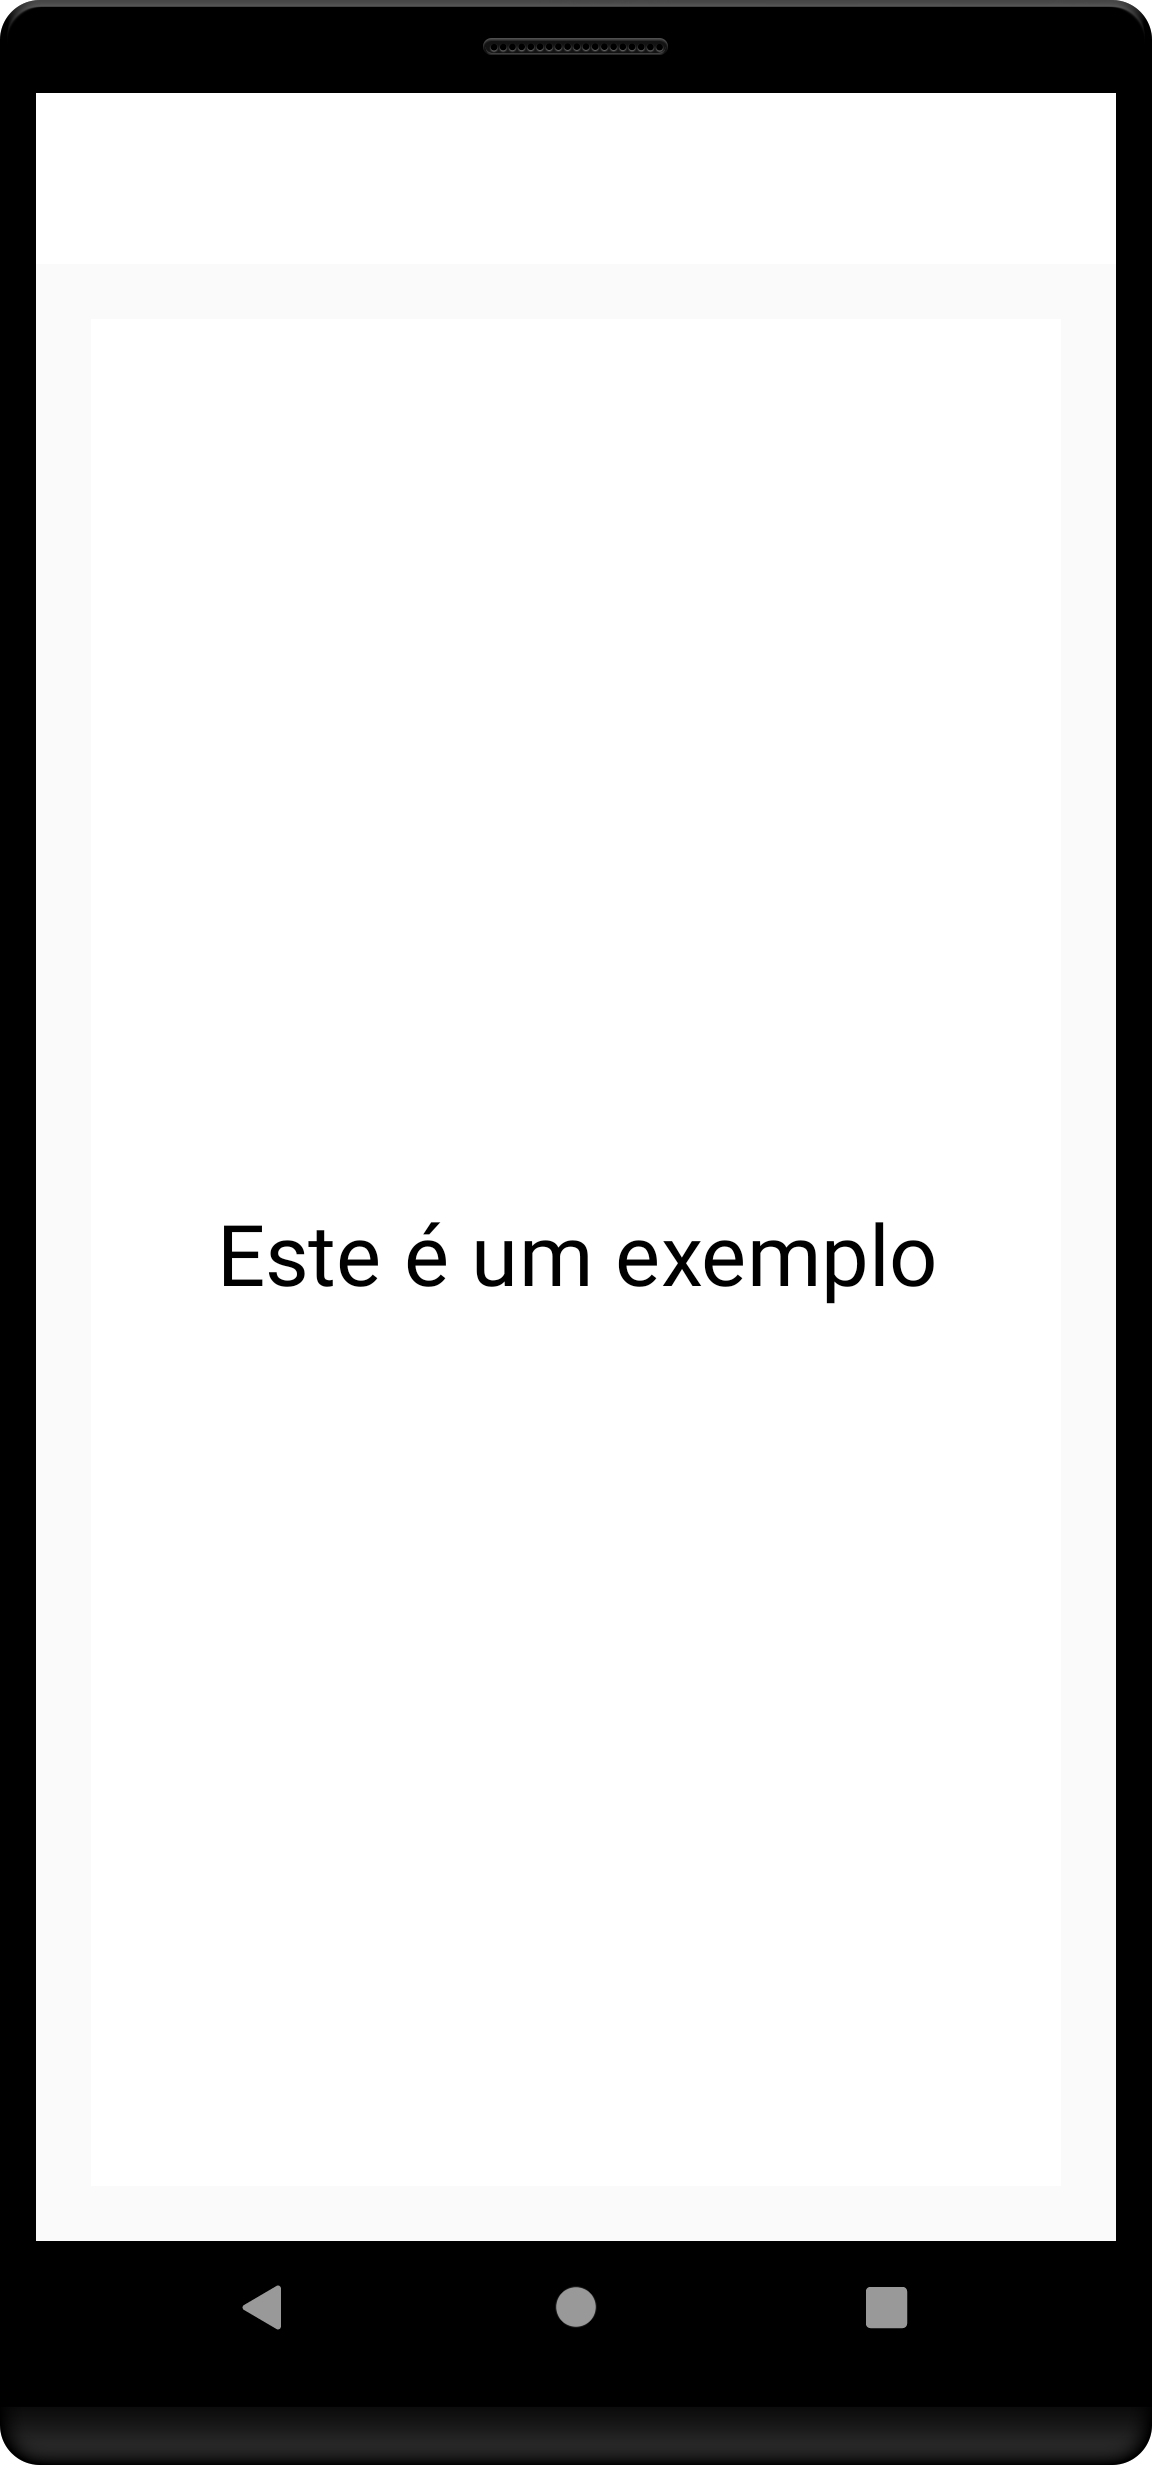
\includegraphics[width=.4\linewidth]{images/screenshots/Android-PinchZoom-zoomed.png}}
	\caption[Componente \textit{PinchZoom} no \textit{Android}]{Exemplo de utilização do componente \textit{PinchZoom} no \textit{Android}}
	\label{fig:pinchZoomAndroidExample}
	\legend{Fonte: Próprio Autor}
\end{figure}


\subsection{Componente \textit{SeekBarZoom}}

O componente \textit{SeekBarZoom} permite que, através de um componente conhecido como \textit{Slider}. O \textit{Slider} é uma barra horizontal com um seletor que desliza da esquerda para a direita, neste caso, utilizado para permitir o ajuste do nível de aproximação de uma tela, sendo a esquerda o menor nível de aproximação da tela, e a direita, o maior.

\begin{figure}[H]
	\begin{center}
		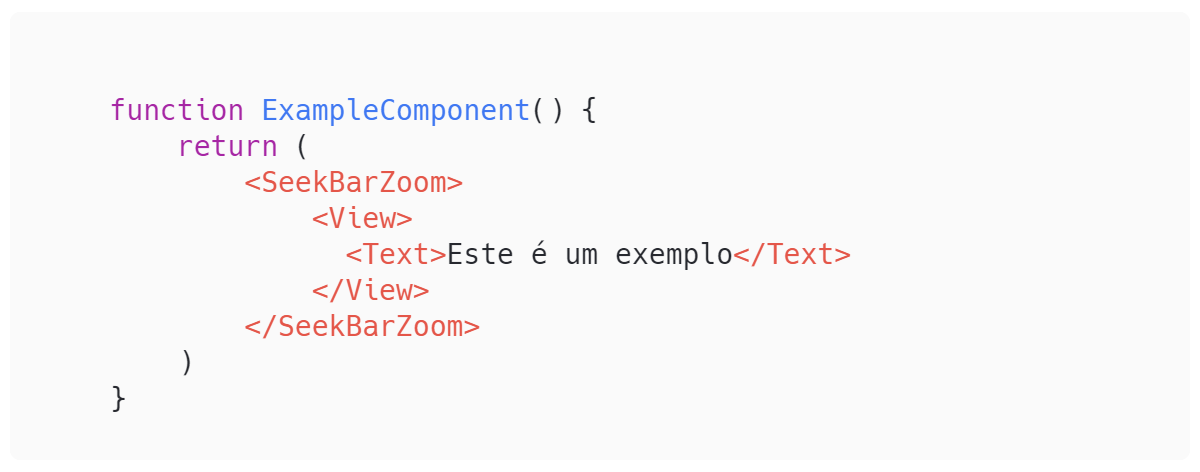
\includegraphics[width=.8\linewidth]{images/SeekBarZoom.png}
		\caption[Componente \textit{SeekBarZoom}]{Exemplo de utilização do componente \textit{SeekBarZoom}}
		\label{fig:seekBarZoomExample}
		\legend{Fonte: Próprio Autor}
	\end{center}
\end{figure}

\par

A seguir, temos os exemplos da utilização do componente \textit{SeekBarZoom} em uma aplicação sendo executada nos sistemas operacionais \textit{iOS} e \textit{Android}

\begin{figure}[H]
	\centering
	\subfloat[Estado inicial do componente \textit{SeekBarZoom}]{
		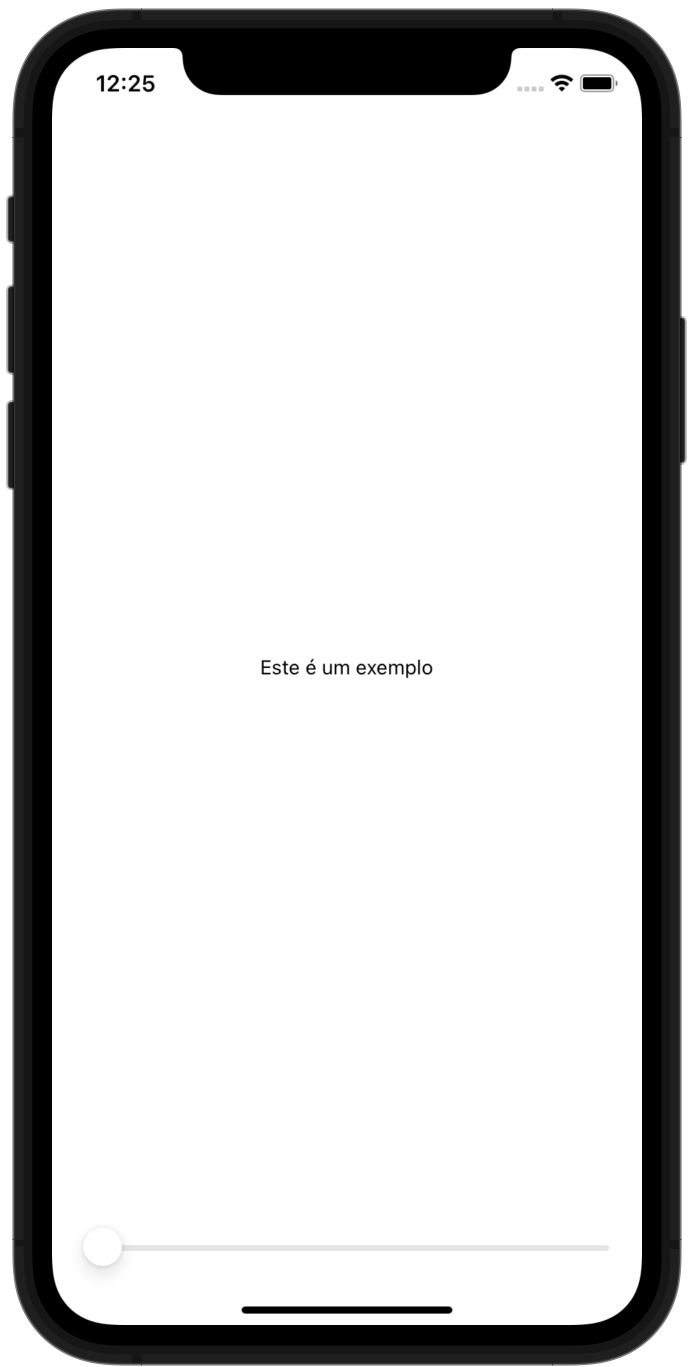
\includegraphics[width=.4\linewidth]{images/screenshots/iOS-SeekBarZoom-initial.png}}
	\hfill
	\subfloat[Estado do componente \textit{SeekBarZoom}após o ajuste de aproximação com o \textit{Slider}]{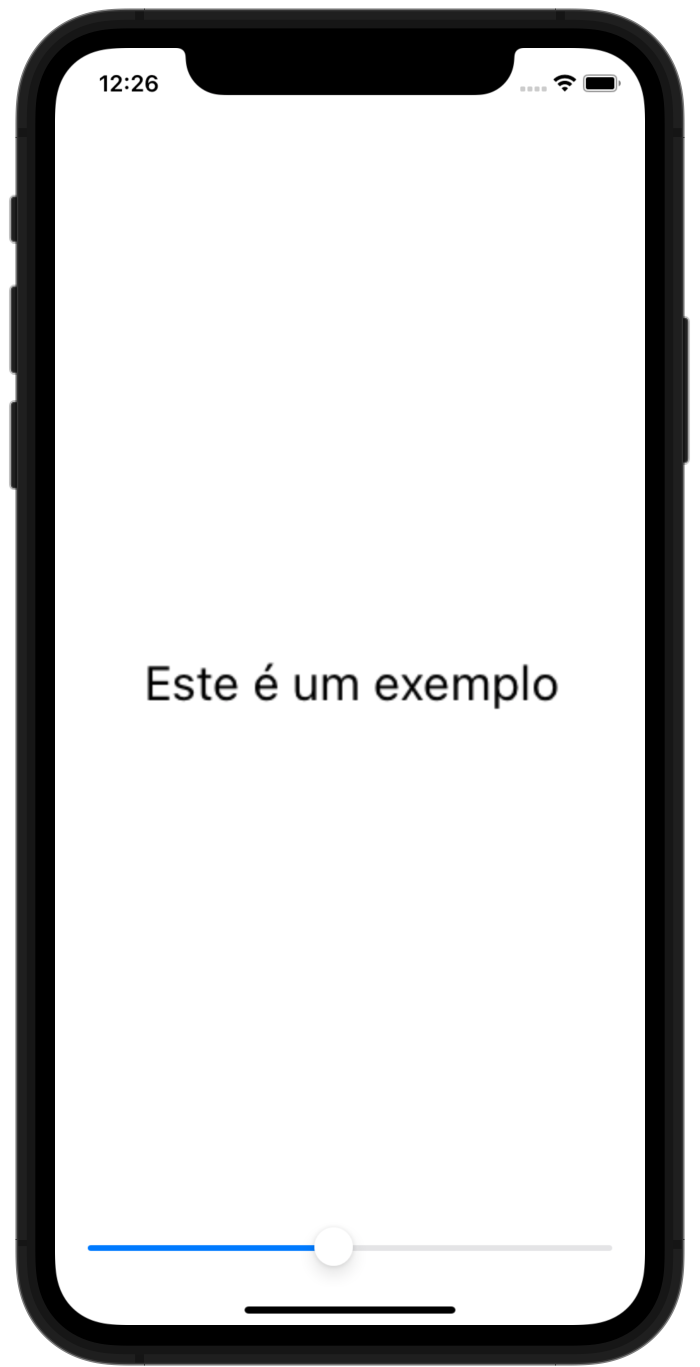
\includegraphics[width=.4\linewidth]{images/screenshots/iOS-SeekBarZoom-zoomed.png}}
	\caption[Componente \textit{SeekBarZoom} no \textit{iOS}]{Exemplo de utilização do componente \textit{SeekBarZoom} no \textit{iOS}}
	\label{fig:seekBarZoomiOSExample}
	\legend{Fonte: Próprio Autor}
\end{figure}

\begin{figure}[H]
	\centering
	\subfloat[Estado inicial do componente \textit{SeekBarZoom}]{
		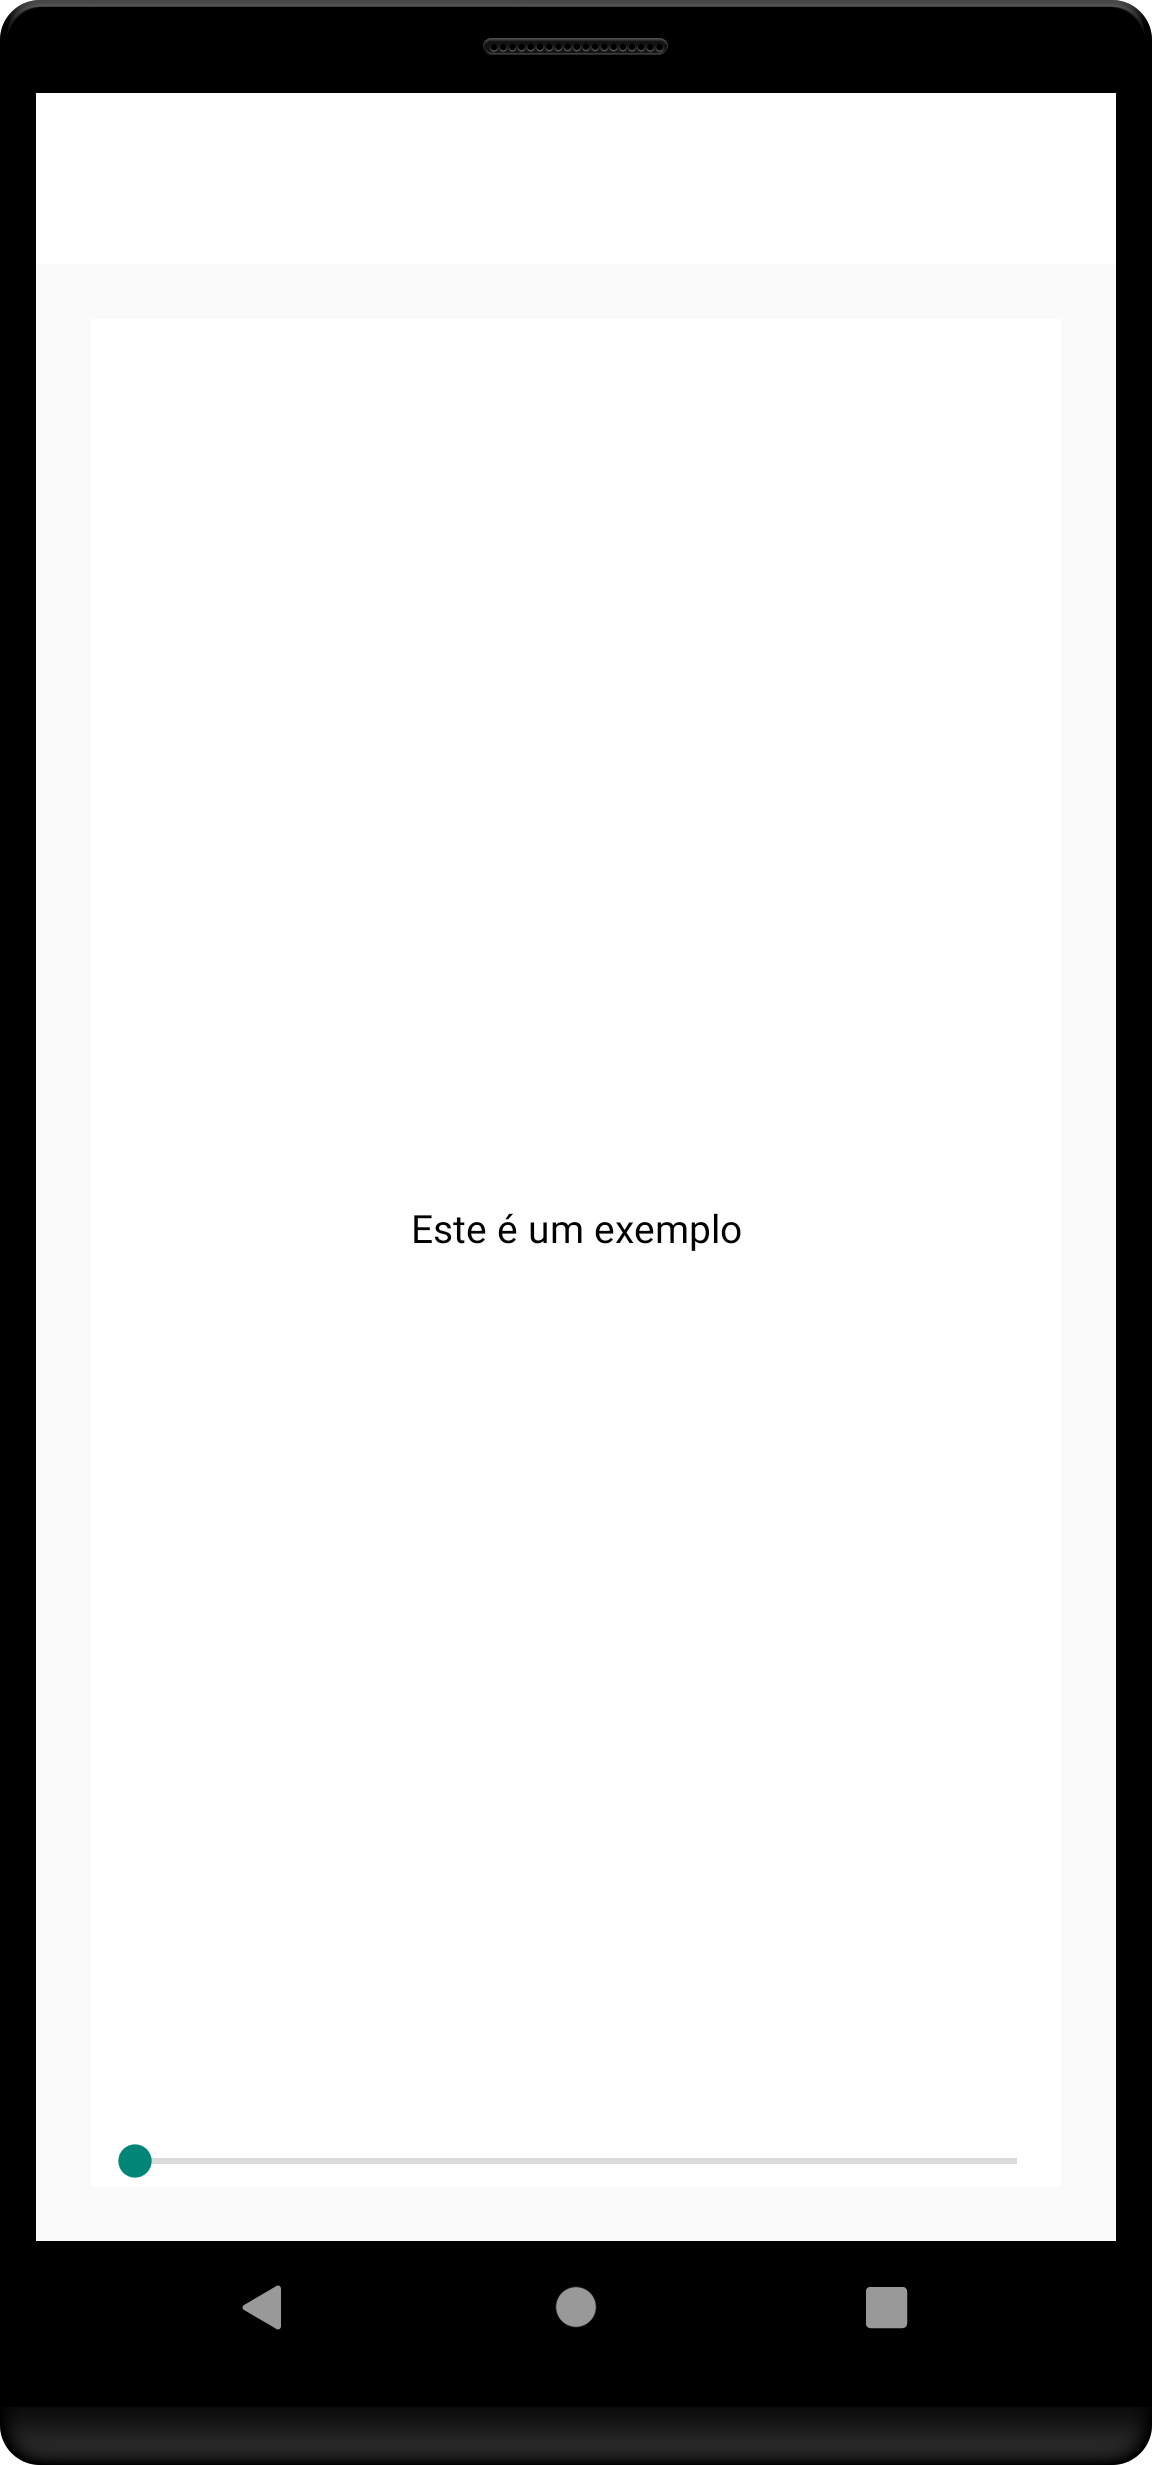
\includegraphics[width=.4\linewidth]{images/screenshots/Android-SeekBarZoom-initial.png}}
	\hfill
	\subfloat[Estado do componente \textit{SeekBarZoom} após o ajuste de aproximação com o \textit{Slider}]{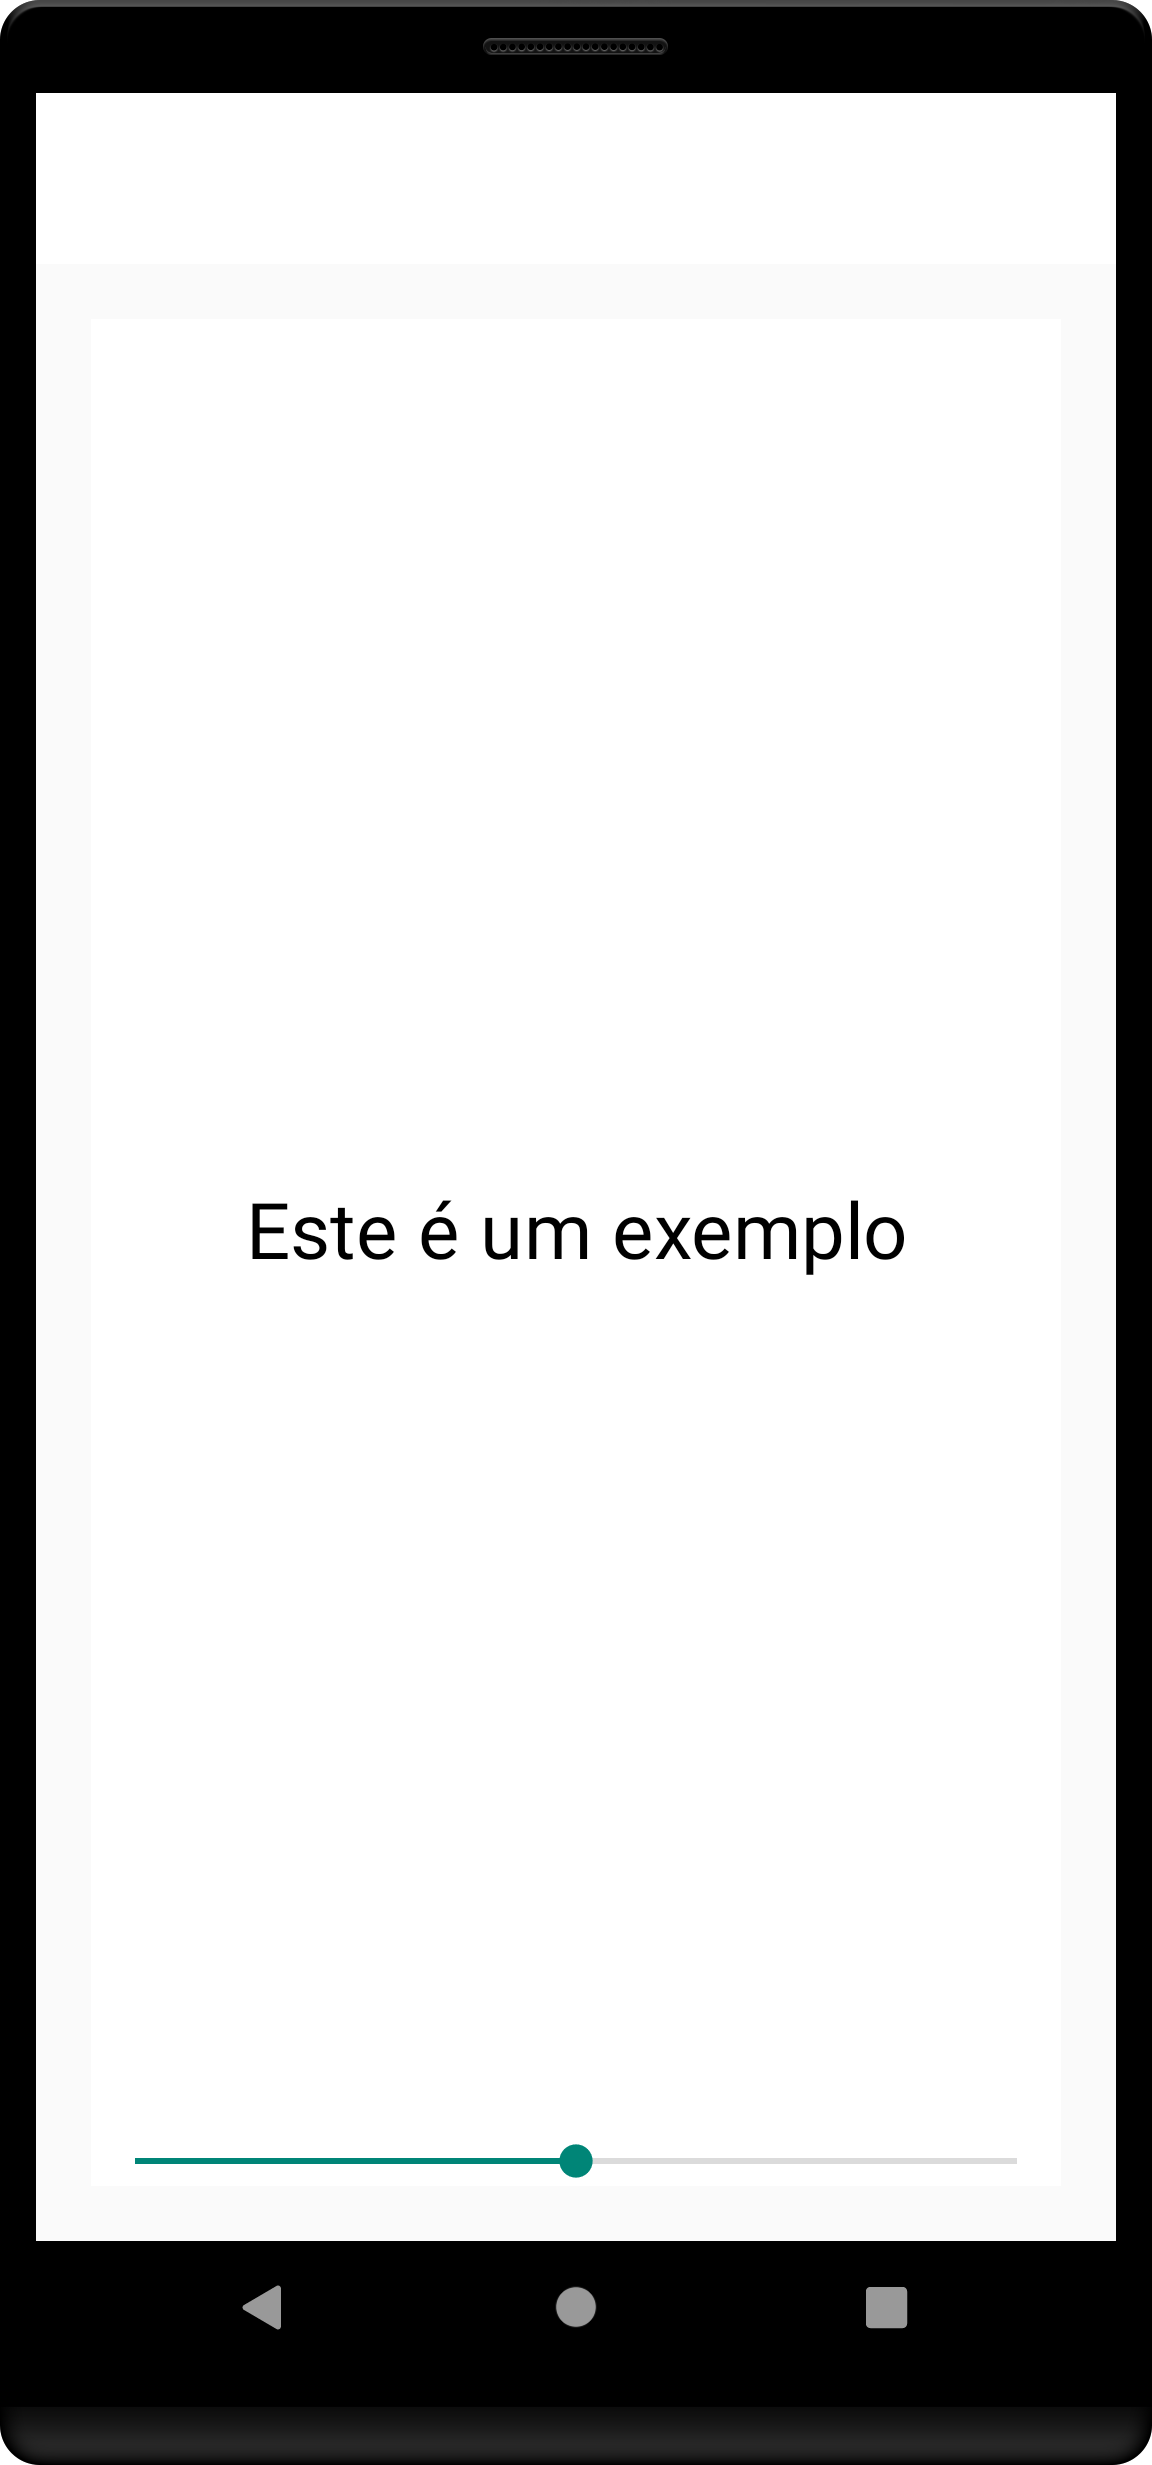
\includegraphics[width=.4\linewidth]{images/screenshots/Android-SeekBarZoom-zoomed.png}}
	\caption[Componente \textit{SeekBarZoom} no \textit{Android}]{Exemplo de utilização do componente \textit{SeekBarZoom} no \textit{Android}}
	\label{fig:seekBarZoomAndroidExample}
	\legend{Fonte: Próprio Autor}
\end{figure}

\subsection{Componente \textit{SimpleRotation}}

Implementar este componente envolveu realizar diversos desafios, como capturar os gestos na tela de um dispositivos até calcular o ângulo de rotação através dos movimentos do dedo na tela. No \textit{ElderlyFrame} este componente não foi completamente implementado, o que dificultou um pouco a sua tradução para \textit{React Native}. Apesar disso, foi possível concluí-lo com sucesso. Abaixo, temos um exemplo de como utilizá-lo:

\begin{figure}[H]
	\begin{center}
		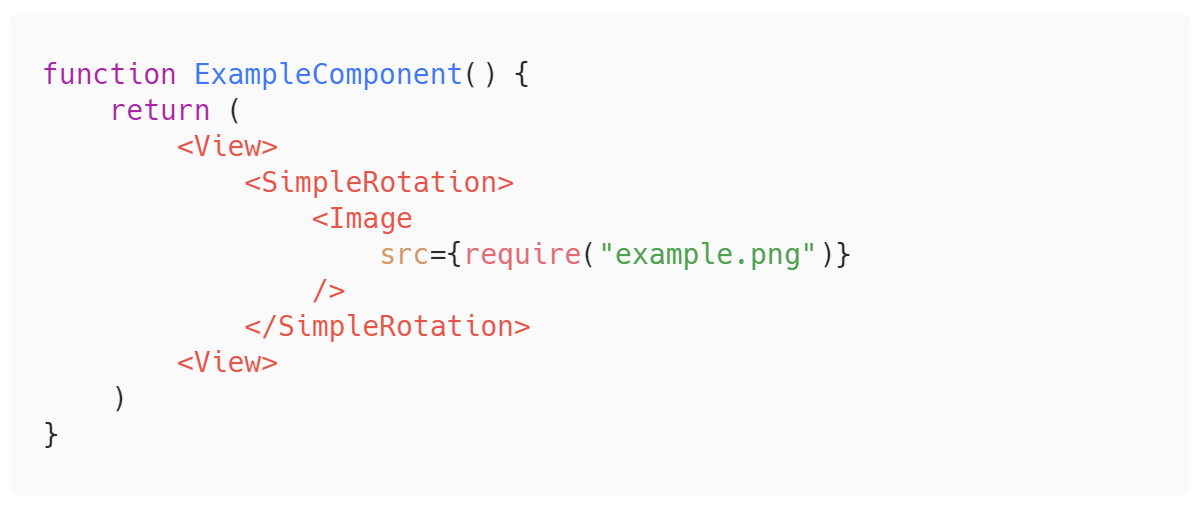
\includegraphics[width=.8\linewidth]{images/SimpleRotation.png}
		\caption[Componente \textit{SimpleRotation}]{Exemplo de utilização do componente \textit{SimpleRotation}}
		\label{fig:simpleRotationExample}
		\legend{Fonte: Próprio Autor}
	\end{center}
\end{figure}

\par

A seguir, temos os exemplos da utilização do componente \textit{SimpleRotation} em uma aplicação sendo executada nos sistemas operacionais \textit{iOS} e \textit{Android}

\begin{figure}[H]
	\centering
	\subfloat[Estado inicial do componente \textit{SimpleRotation}]{
		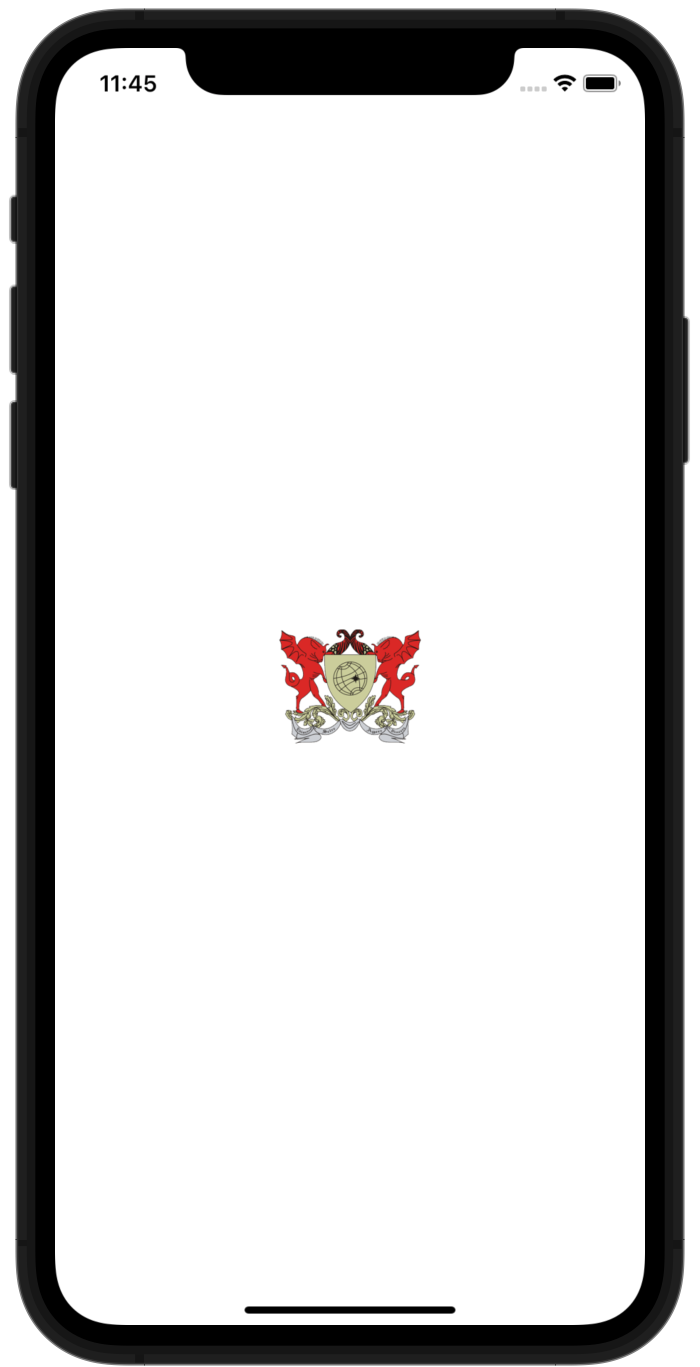
\includegraphics[width=.4\linewidth]{images/screenshots/iOS-SimpleRotation-initial.png}}
	\hfill
	\subfloat[Estado do componente \textit{SimpleRotation} após o movimento de rotação usando apenas o toque com um dedo]{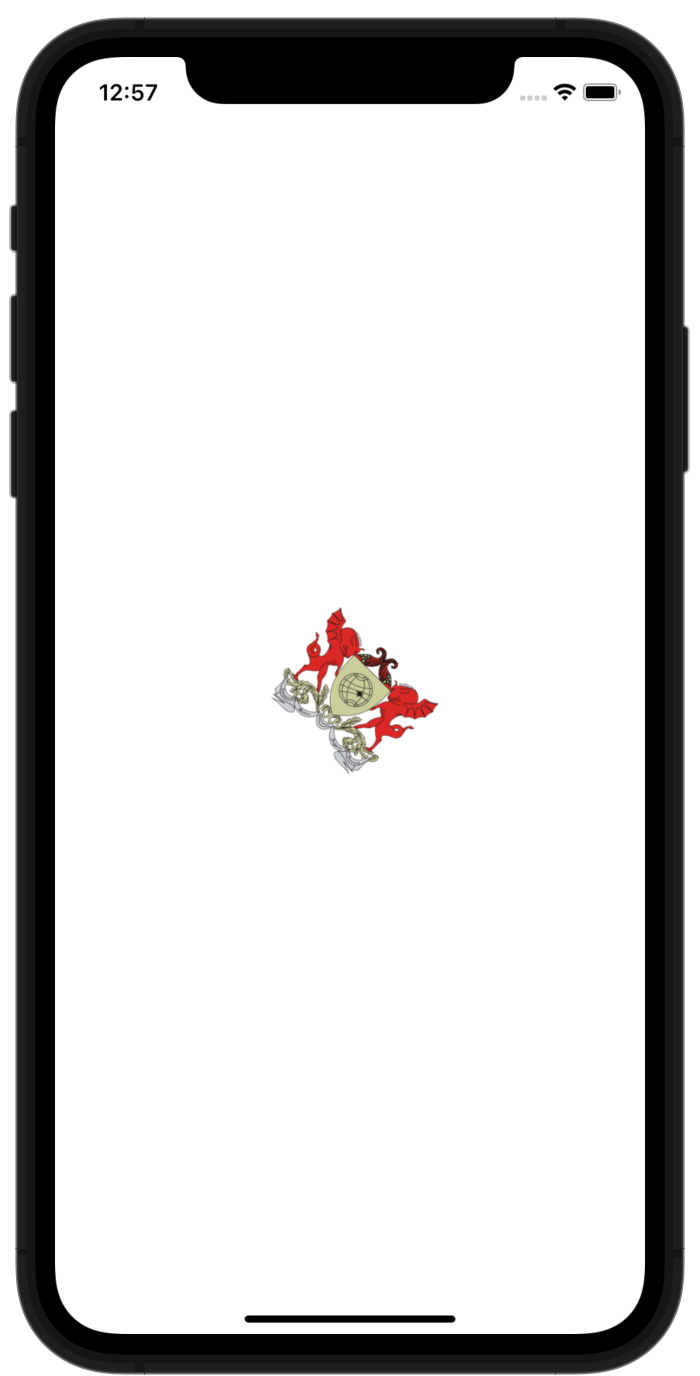
\includegraphics[width=.4\linewidth]{images/screenshots/iOS-SimpleRotation-rotated.png}}
	\caption[Componente \textit{SimpleRotation} no \textit{iOS}]{Exemplo de utilização do componente \textit{SimpleRotation} no \textit{iOS}}
	\label{fig:simpleRotationiOSExample}
	\legend{Fonte: Próprio Autor}
\end{figure}

\begin{figure}[H]
	\centering
	\subfloat[Estado inicial do componente \textit{SimpleRotation}]{
		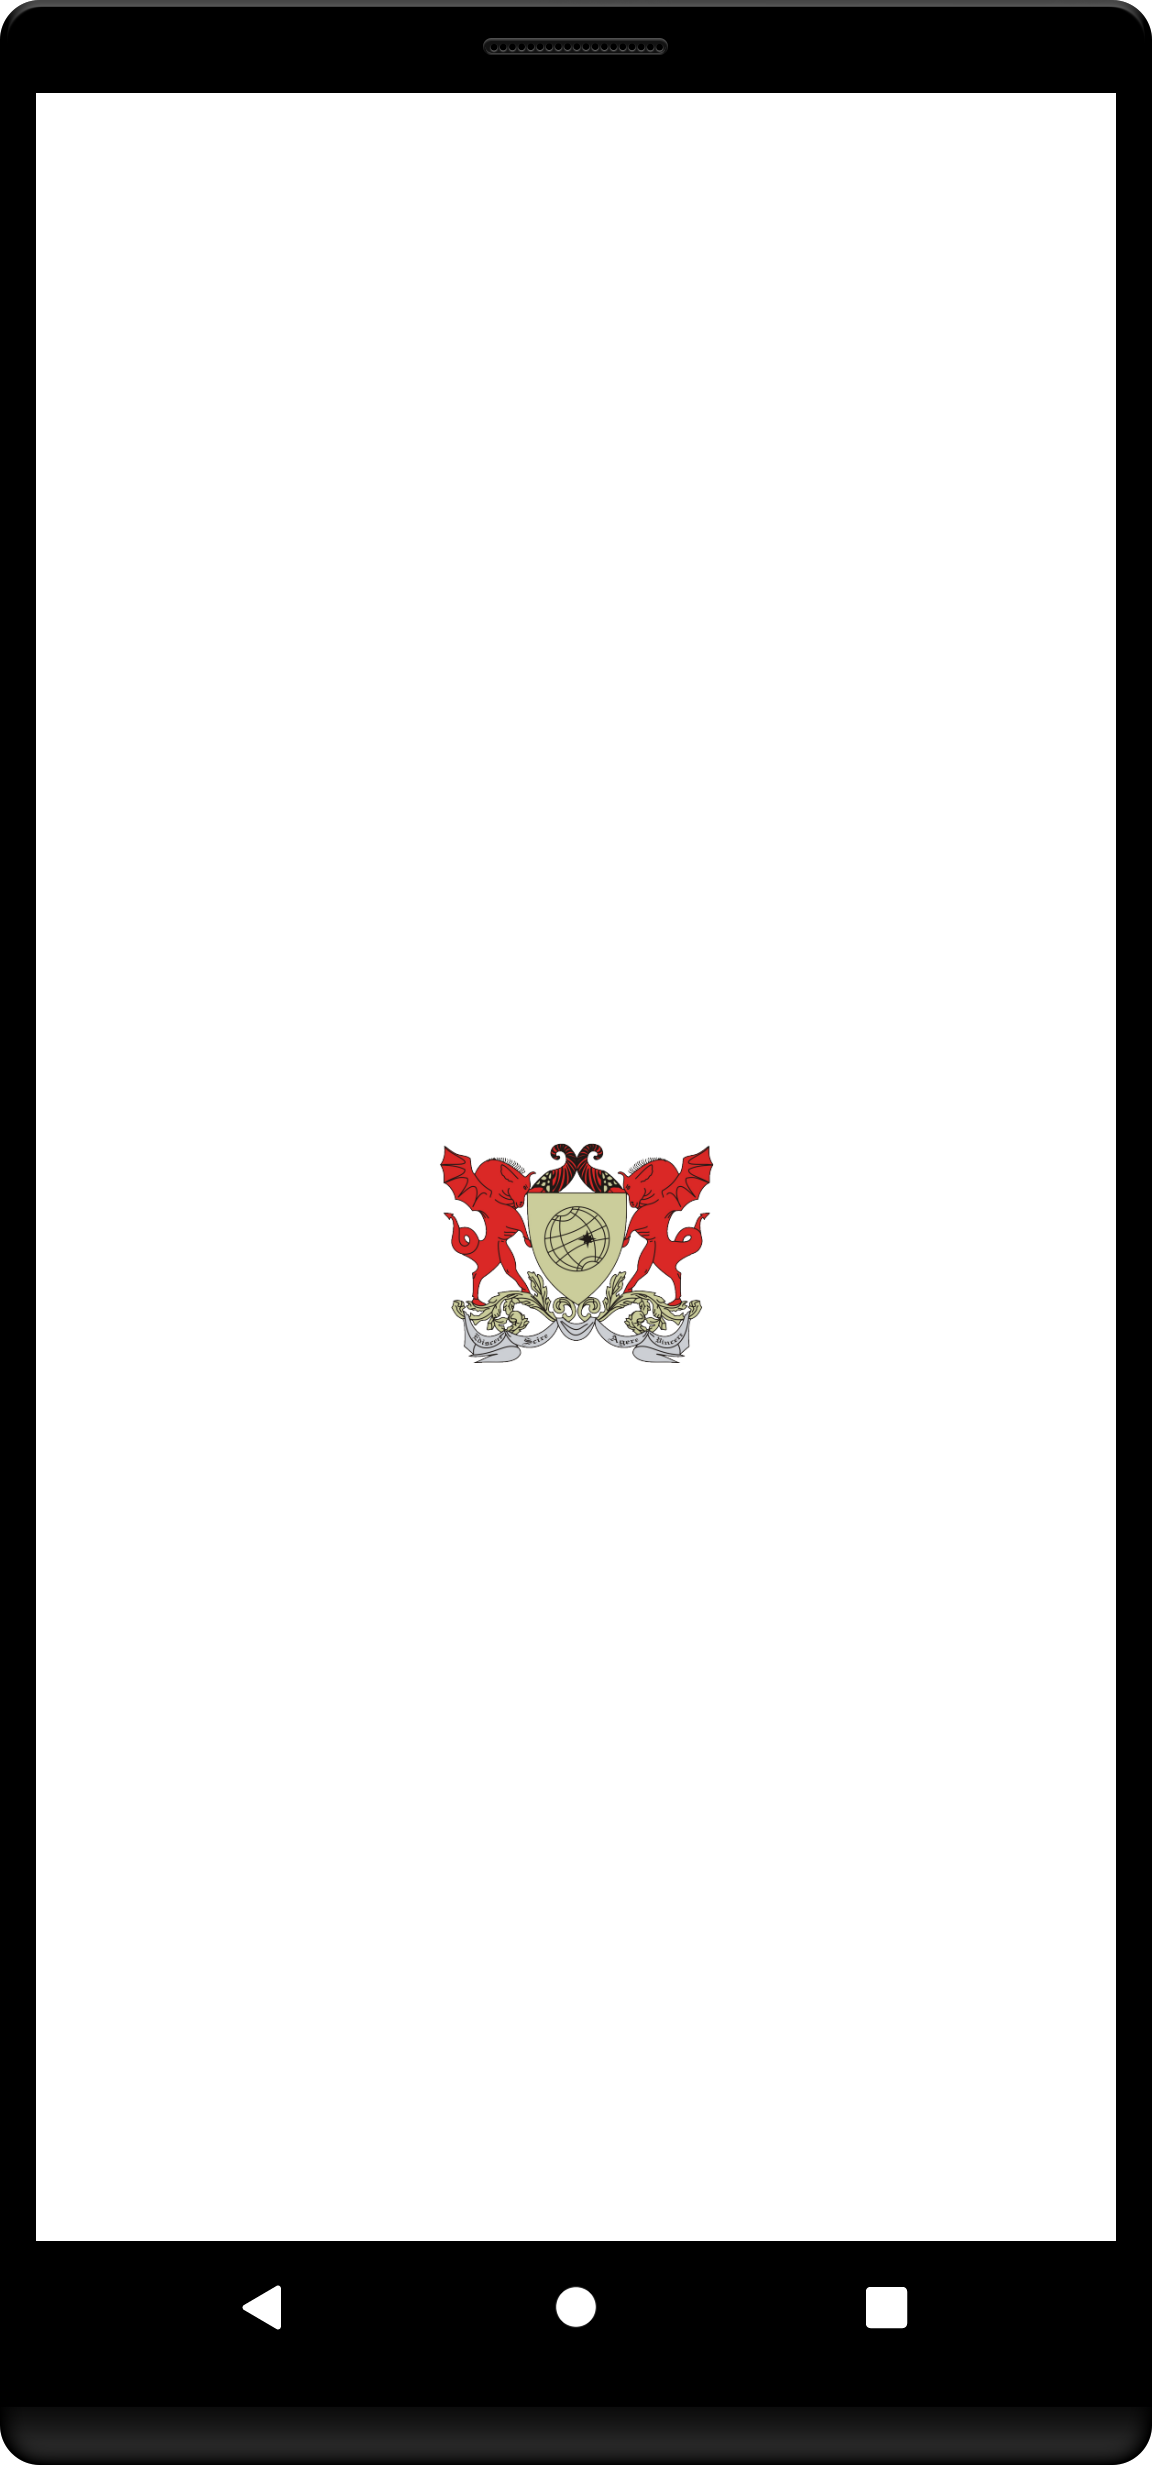
\includegraphics[width=.4\linewidth]{images/screenshots/Android-SimpleRotation-initial.png}}
	\hfill
	\subfloat[Estado do componente \textit{SimpleRotation} após o movimento de rotação usando apenas o toque com um dedo]{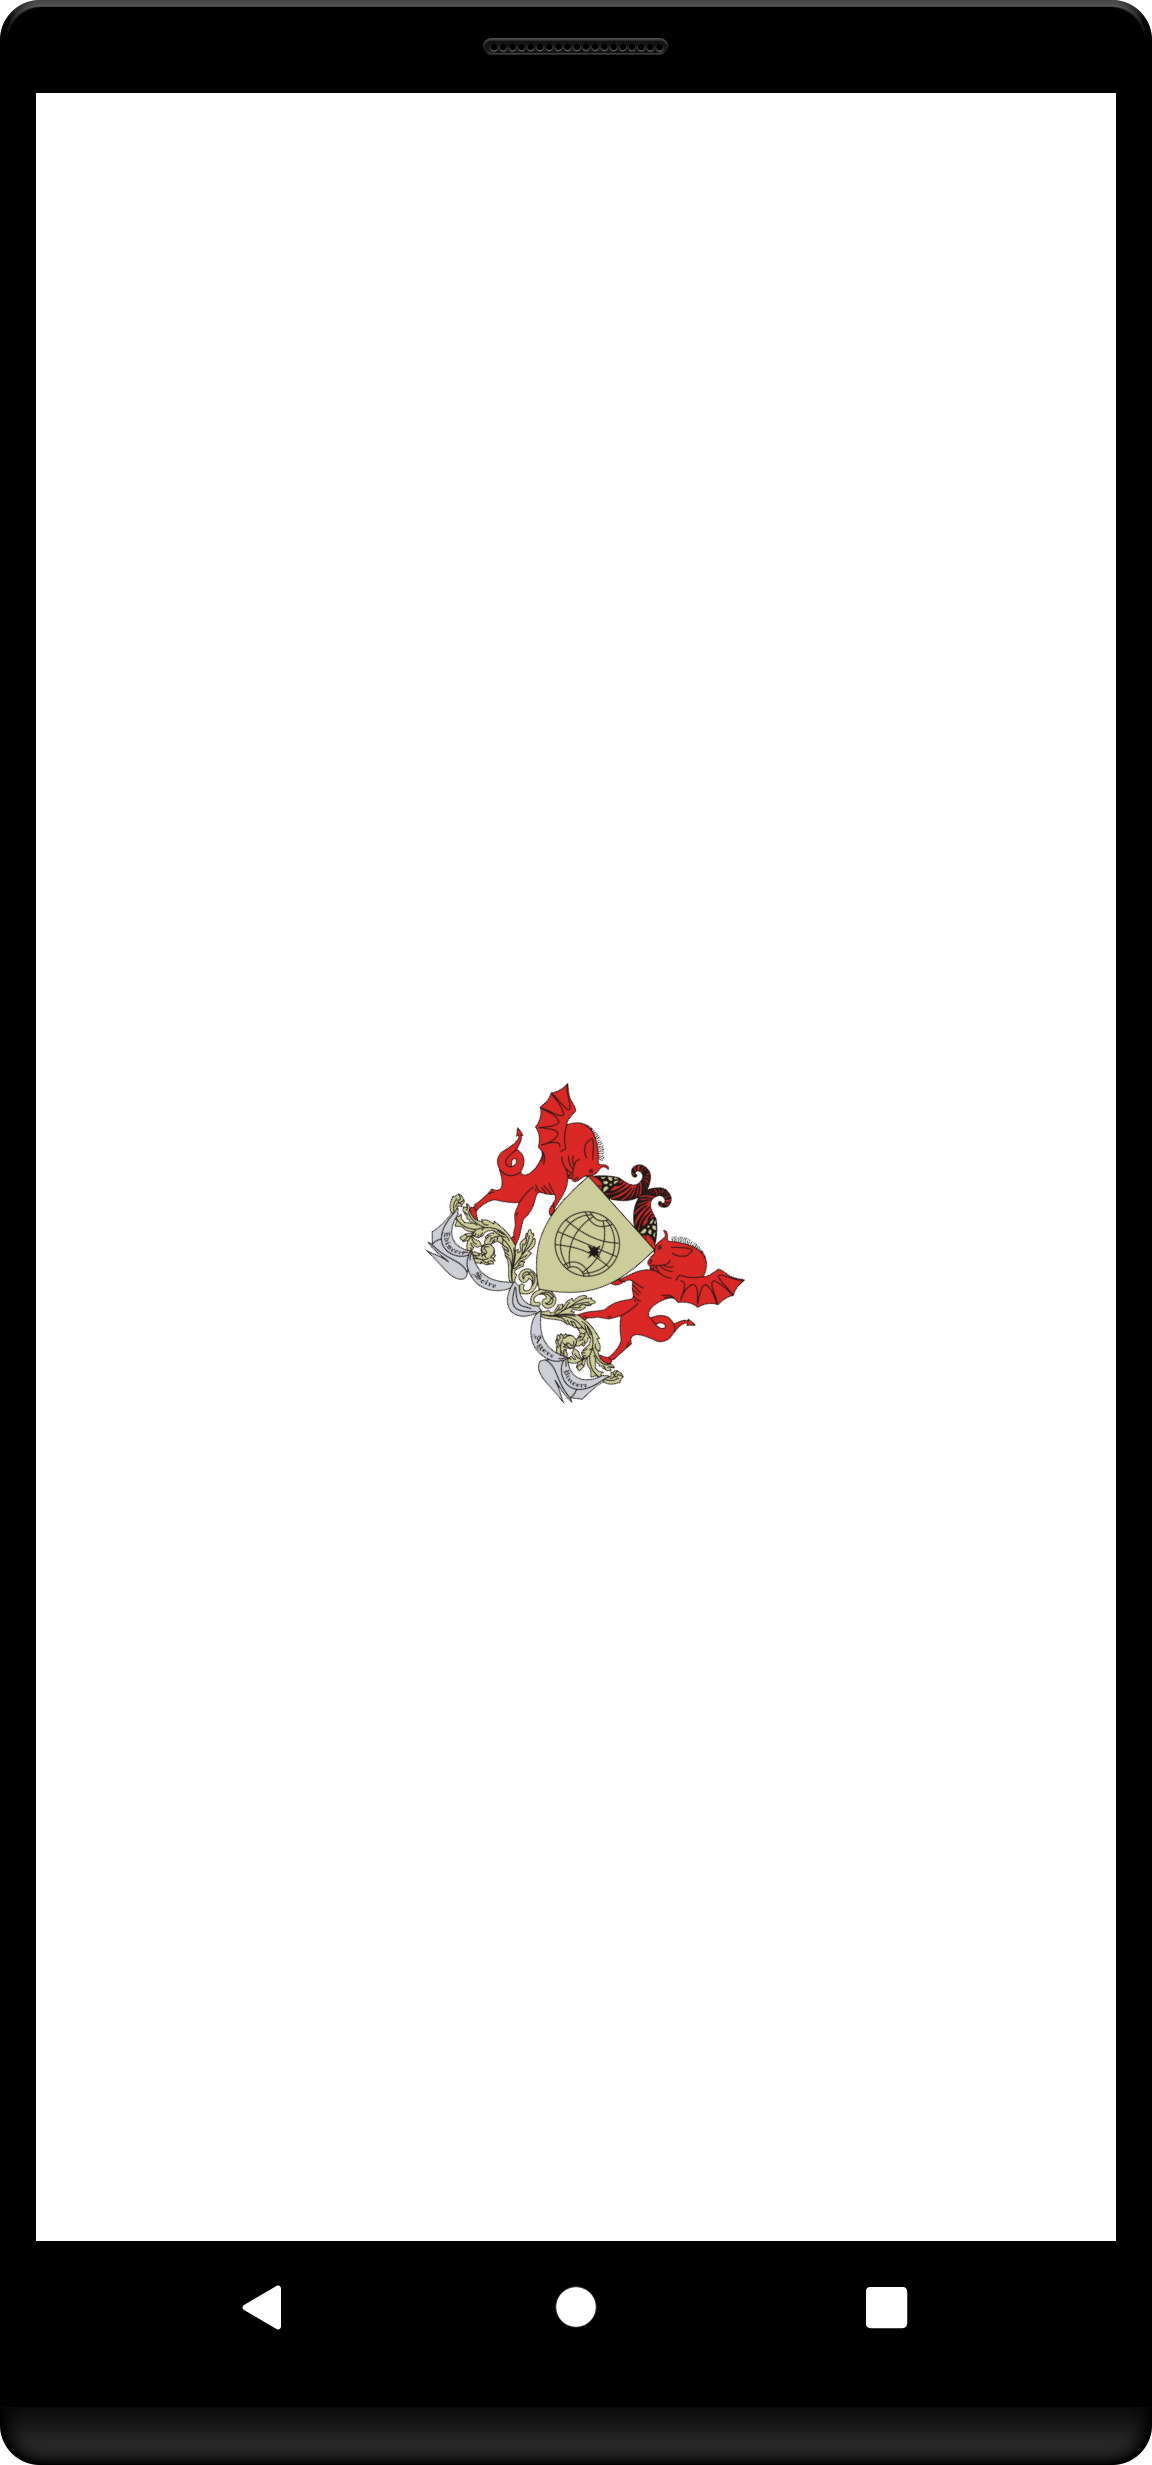
\includegraphics[width=.4\linewidth]{images/screenshots/Android-SimpleRotation-rotated.png}}
	\caption[Componente \textit{SimpleRotation} no \textit{Android}]{Exemplo de utilização do componente \textit{SimpleRotation} no \textit{Android}}
	\label{fig:simpleRotationAndroidExample}
	\legend{Fonte: Próprio Autor}
\end{figure}

\subsection{Componente \textit{SpeechToText}}

O componente \textit{SpeechToText}, originalmente nomeado \textit{SpeechText}, teve seu nome alterado para ser mais descritivo sobre seu propósito. Este elemento permite que, ao pressionar o ícone de microfone, o mecanismo de reconhecimento de voz do dispositivo seja ativado e, a partir de então, tudo o que é dito será convertido para texto e inserido no campo digitável. Abaixo, temos um exemplo de como utilizá-lo no código de uma aplicação:

\begin{figure}[H]
	\begin{center}
		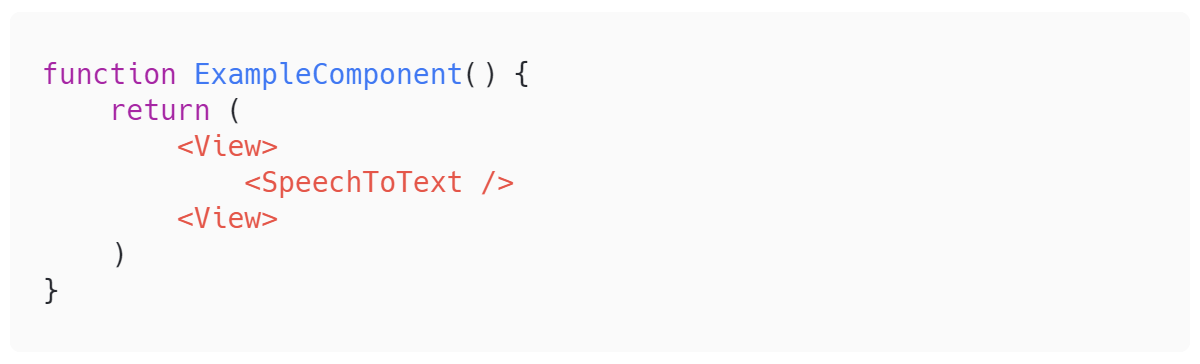
\includegraphics[width=.8\linewidth]{images/SpeechToText.png}
		\caption[Componente \textit{SpeechToText}]{Exemplo de utilização do componente \textit{SpeechToText}}
		\label{fig:speechToTextExample}
		\legend{Fonte: Próprio Autor}
	\end{center}
\end{figure}


\par

A seguir, temos os exemplos da utilização do componente \textit{SpeechToText} em uma aplicação sendo executada nos sistemas operacionais \textit{iOS} e \textit{Android}

\begin{figure}[H]
	\centering
	\subfloat[Estado inicial do componente \textit{SpeechToText}]{
		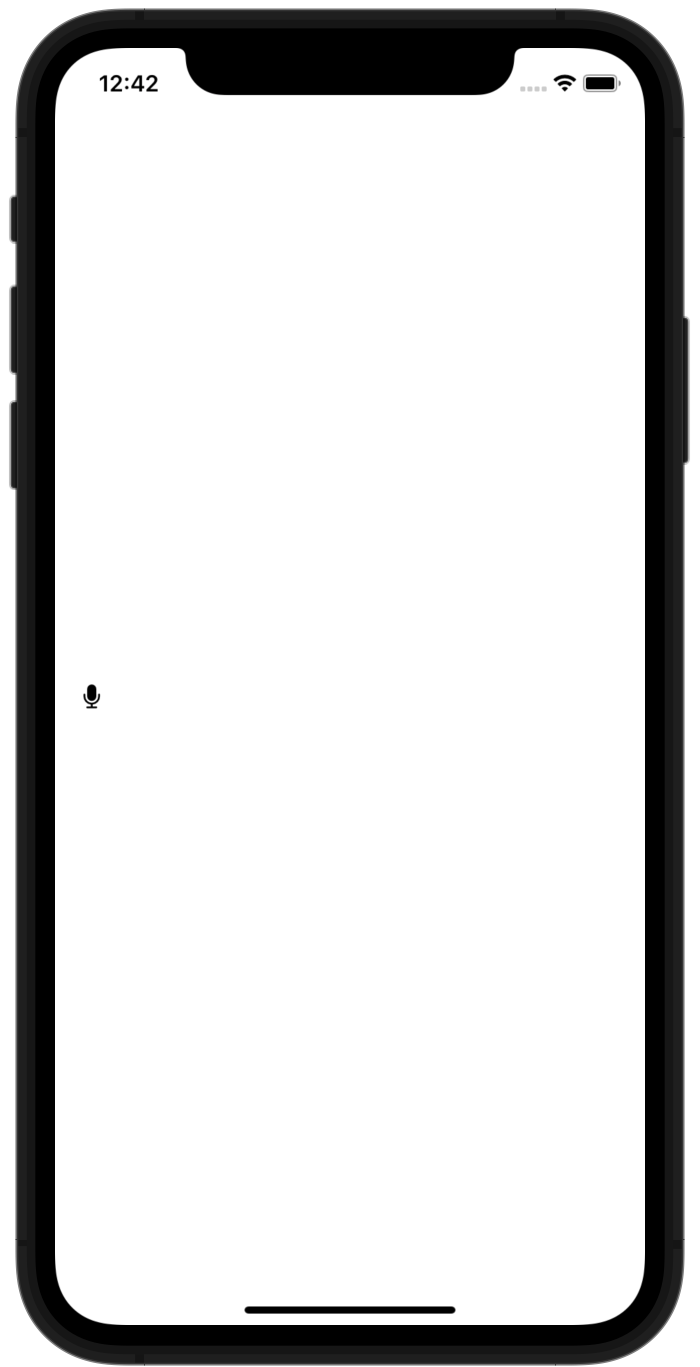
\includegraphics[width=.4\linewidth]{images/screenshots/iOS-SpeechToText-empty.png}}
	\hfill
	\subfloat[Estado do componente \textit{SpeechToText} após o reconhecimento de voz]{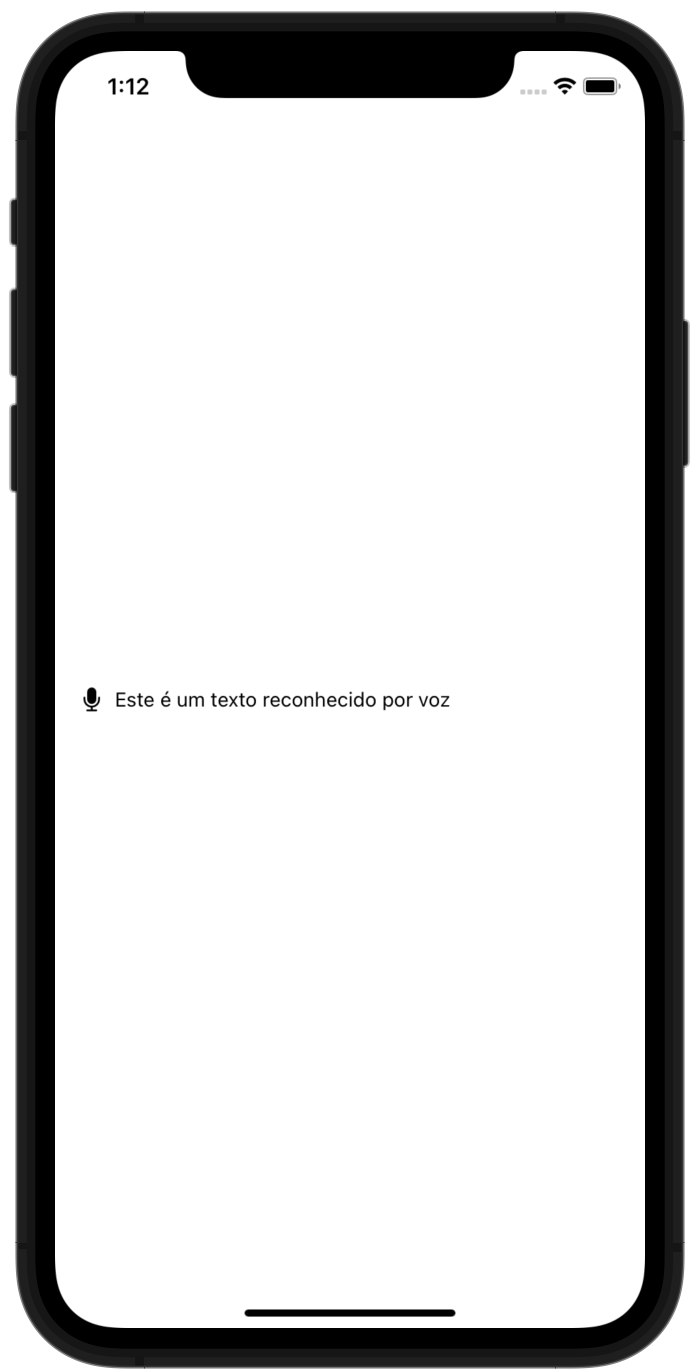
\includegraphics[width=.4\linewidth]{images/screenshots/iOS-SpeechToText-recognized.png}}
	\caption[Componente \textit{SpeechToText} no \textit{iOS}]{Exemplo de utilização do componente \textit{SpeechToText} no \textit{iOS}}
	\label{fig:speechToTextiOSExample}
	\legend{Fonte: Próprio Autor}
\end{figure}

\begin{figure}[H]
	\centering
	\subfloat[Estado inicial do componente \textit{SpeechToText}]{
		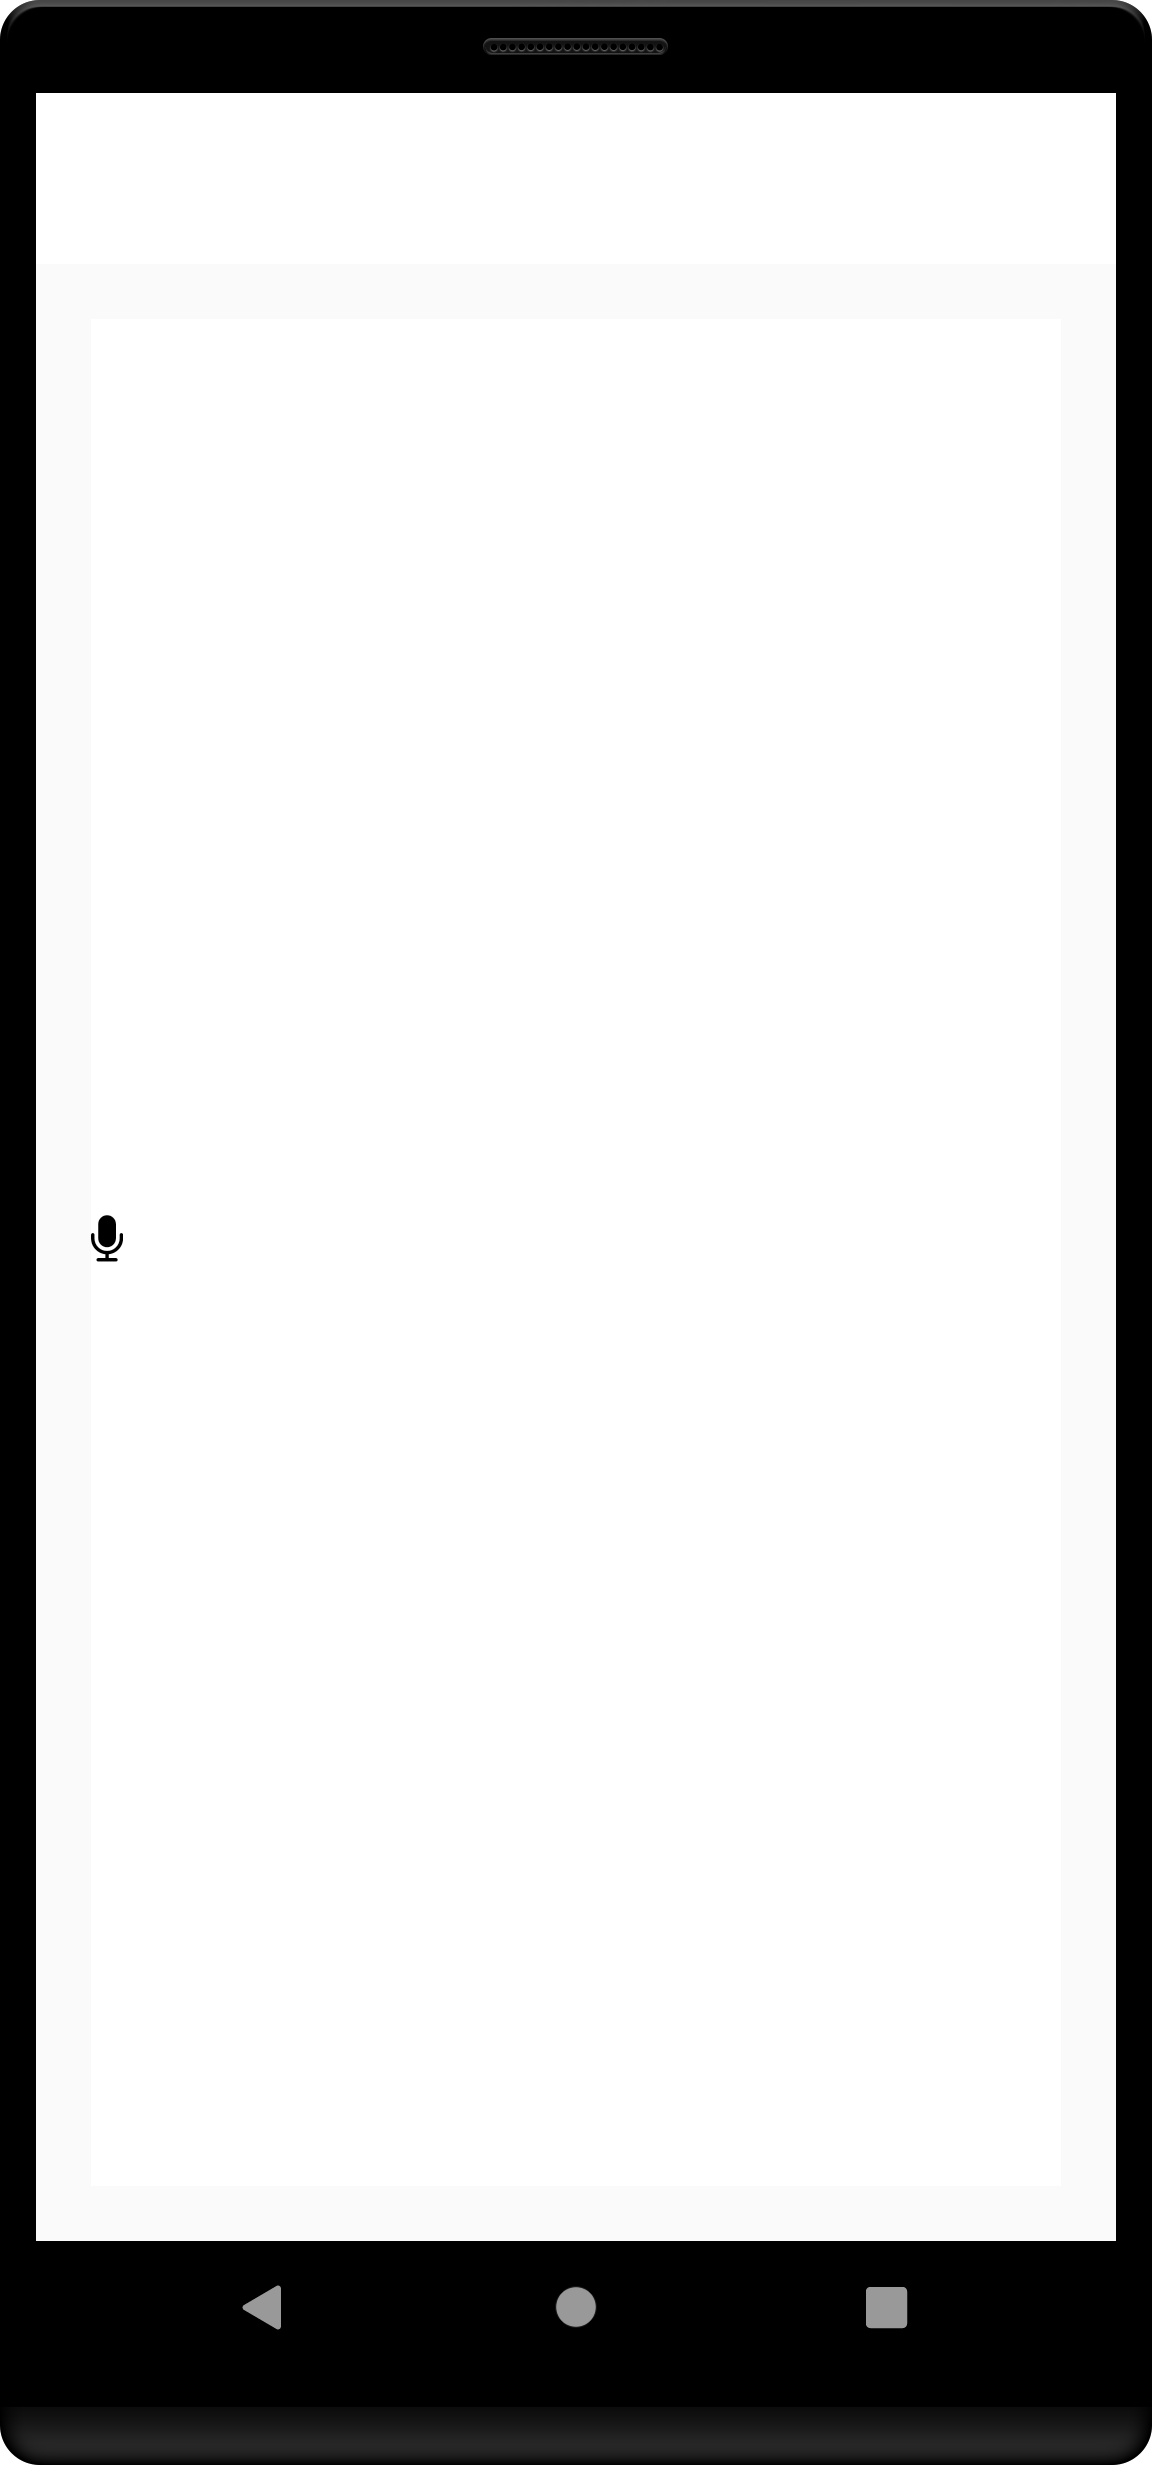
\includegraphics[width=.4\linewidth]{images/screenshots/Android-SpeechToText-empty.png}}
	\hfill
	\subfloat[Estado do componente \textit{SpeechToText} após o reconhecimento de voz]{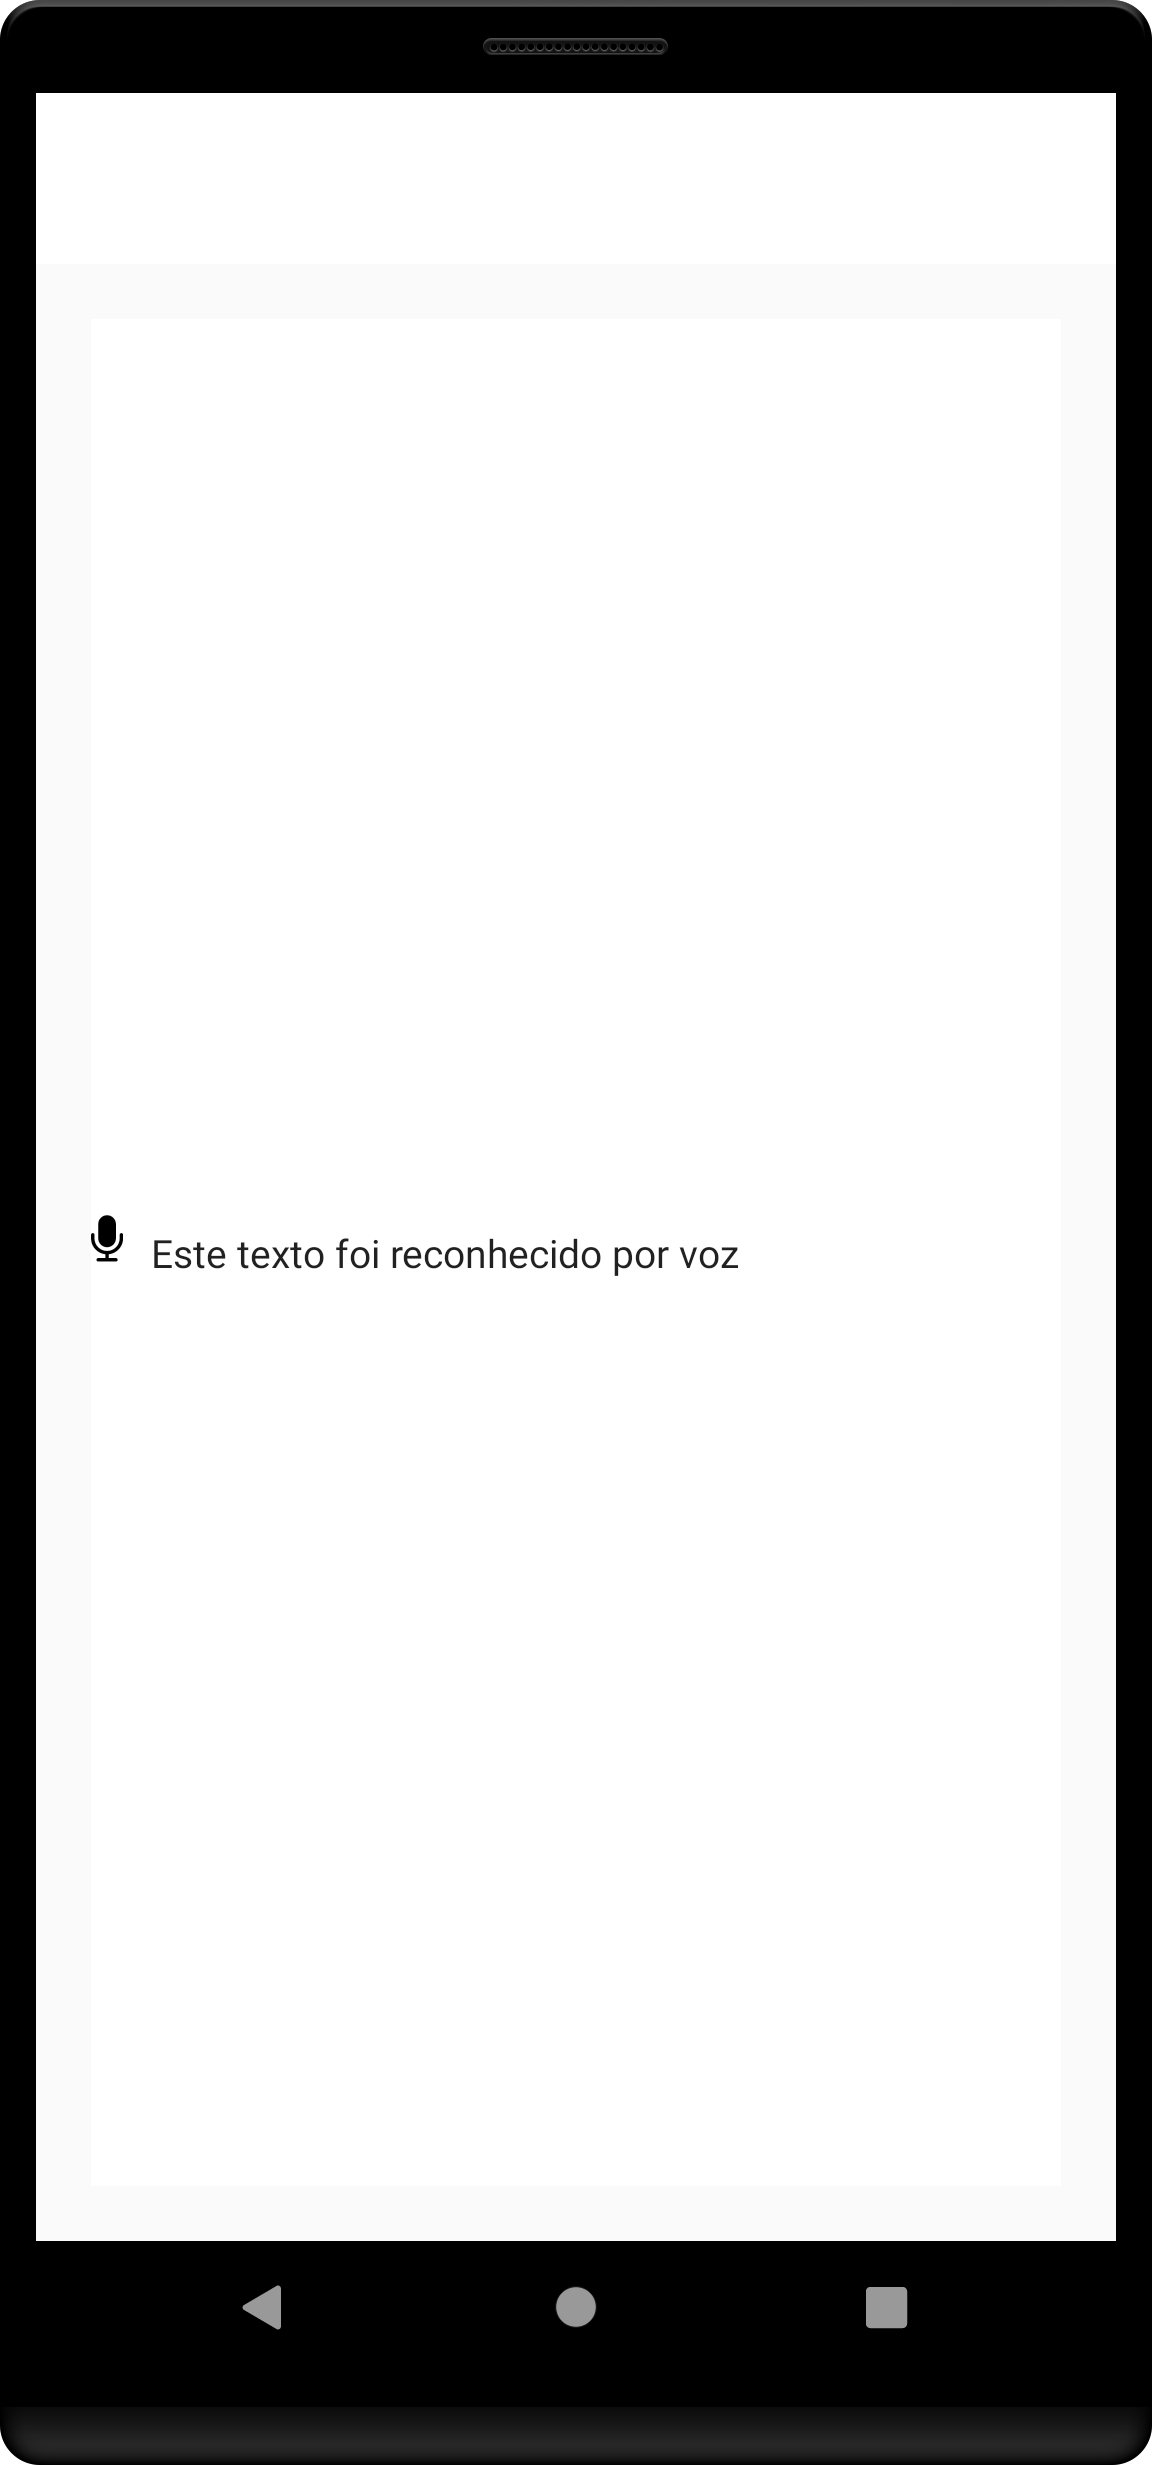
\includegraphics[width=.4\linewidth]{images/screenshots/Android-SpeechToText-recognized.png}}
	\caption[Componente \textit{SpeechToText} no \textit{Android}]{Exemplo de utilização do componente \textit{SpeechToText} no \textit{Android}}
	\label{fig:speechToTextAndroidExample}
	\legend{Fonte: Próprio Autor}
\end{figure}

\subsection{Componente \textit{TouchZoom}}

O componente \textit{TouchZoom}, permite que a tela de uma aplicação seja aproximada ao realizar um toque mais longo na tela de um dispositivo. Dessa forma, dispensa que a pessoa que interage com o dispositivo realize movimentos mais complexos, como toques com múltiplos dedos. Abaixo, temos um exemplo de como utilizá-lo no código de uma aplicação:

\begin{figure}[H]
	\begin{center}
		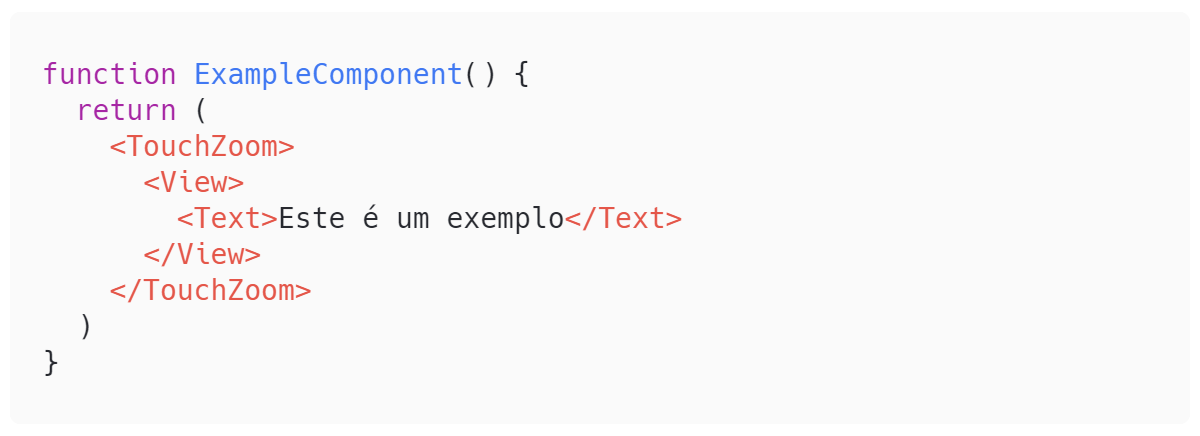
\includegraphics[width=.8\linewidth]{images/TouchZoom.png}
		\caption[Componente \textit{TouchZoom}]{Exemplo de utilização do componente \textit{TouchZoom}}
		\label{fig:touchZoomExample}
		\legend{Fonte: Próprio Autor}
	\end{center}
\end{figure}


\section{Pacote no \textit{npm}}

Como dito anteriormente, a forma escolhida para disponibilizar este framework para ser usado em aplicações para dispositivos móveis foi através do \textit{npm}. Para adicionar o framework à uma aplicação construída usando \textit{React Native} basta utilizar um dos comandos abaixo no terminal, dentro da pasta raiz do seu projeto:

\begin{lstlisting}[language=bash]
# Caso use o npm
$ npm install react-native-accessibility-elderly

# Caso use o yarn
$ yarn add react-native-accessibility-elderly
\end{lstlisting}

Pode ser necessário executar o comando \textit{link} para que as bibliotecas de terceiros possam ser devidamente encontradas, a depender da versão do \textit{React Native} usada no projeto, visto que as versões mais recentes(0.60 ou superior) não requerem a execução manual deste comando. Execute o comando abaixo no terminal, dentro da pasta raiz do seu projeto:

\begin{lstlisting}[language=bash]t
$ react-native link
\end{lstlisting}

\chapter{Conclusão e Trabalhos Futuros}\label{sec:futuro}

Conclui-se que os resultados finais deste projeto foram satisfatórios, visto que foi possível cobrir as especificações do projeto base, \textit{ElderlyFrame}. Além disso, também foi possível testar e garantir que é possível utilizar o artefato produzido para construir uma aplicação multiplataforma utilizando \textit{React Native}.

Como trabalhos futuros, vê-se a necessidade de acompanhar a evolução da tecnologia utilizada, no caso, \textit{React Native}, pois a mesma constantemente recebe melhorias e correções que podem ter impacto direto na usabilidade desta ferramenta.

Reduzir a utilização de bibliotecas de terceiros seria outro ponto a se considerar, pois eventualmente algumas delas podem deixar de receber suporte, e se tornarem inutilizáveis. Portanto, é desejável que se tenha o mínimo de dependências. Seria possível, por exemplo, implementar o \textit{Slider} do componente \textit{SeekBarZoom} apenas utilizando a biblioteca \textit{react-native-gesture-handler}, eliminando assim a dependência \textit{@react-native-community/slider}.

A realização de uma pesquisa para validação da eficiência dos componentes implementados neste trabalho seria de grande utilidade. Assim como foi feito pela \Cite{tesedamaris}, para dar início ao \textit{ElderlyFrame}, validar os resultados junto a grupos de idosos permitiria verificar se este \textit{framework} cumpriu seu propósito.

\par

Inicialmente foi proposta a criação de uma documentação interativa usando a ferramenta \textit{Storybook}. Porém, a mesma apresentou alguns problemas que demandariam muito tempo para serem solucionados, e, dentro do prazo estabelecido, não seria viável. Um código bem documentado facilita para que outras pessoas possam utilizá-lo da maneira correta. Desta forma, criar esta documentação é vista como de suma importância e como trabalho a ser realizado no futuro.

\chapter{Cronograma}\label{sec:cronograma}

Para execução deste projeto, foram estabelecidas as atividades a serem realizadas e os meses que em que irão ocorrer durante o período deste projeto. O quadro a seguir apresenta essa relação:

\par

\begin{table}[htbp]
	\centering
	\caption[Cronograma mensal]{Cronograma do Projeto em Meses}
	\label{tab:cronogramaMensal}
	\begin{tabular}{lcccccccc} %|c|c|c|c|c|c|c|c|c|c|c|c
		\toprule
		\textbf{Atividade} & \textbf{1} & \textbf{2} & \textbf{3} & \textbf{4} & \textbf{5} & \textbf{6} & \textbf{7} & \textbf{8} \\
		\midrule
		Análise do Tema    & $\bullet$  & $\bullet$  &            &            &            &            &            &            \\
		Revisão Literária  &            & $\bullet$  & $\bullet$  &            &            & $\bullet$  & $\bullet$  &            \\
		Implementação      &            & $\bullet$  & $\bullet$  & $\bullet$  & $\bullet$  & $\bullet$  & $\bullet$  &            \\
		Documentação       &            &            & $\bullet$  & $\bullet$  & $\bullet$  & $\bullet$  & $\bullet$  & $\bullet$  \\
		Monografia         &            &            & $\bullet$  & $\bullet$  & $\bullet$  & $\bullet$  & $\bullet$  & $\bullet$  \\
		Testes             &            &            &            &            &            & $\bullet$  & $\bullet$  & $\bullet$  \\
		\bottomrule
	\end{tabular}
	\fonte{Próprio Autor}
\end{table}

As demandas de tempo(em horas) estimadas para orientação, desenvolvimento e revisão da literatura, do projeto escrito e demais artefatos produzidos são:

\par

\begin{table}[htpb]
	\centering
	\caption[Cronograma em horas]{Estimativa de tempo para cada atividade}
	\label{tab:cronogramaHoras}
	\begin{tabular}{lcc}
		\toprule
		\textbf{Item} & \textbf{Custeio} & \textbf{Tempo(horas)} \\
		\midrule
		Orientação    & Governo Federal  & 40                    \\
		Projeto       & Próprio          & 300                   \\
		Revisão       & Próprio          & 20                    \\
		\bottomrule
		Total         &                  & 360
	\end{tabular}
	\fonte{Próprio autor}
\end{table}

\chapter{Orçamento}\label{sec:orcamento}

Estão orçados para este projeto os itens contidos na tabela abaixo, acompanhados de seus respectivos financiadores e valores:

\par

\begin{table}[htpb]
	\centering
	\caption[Orçamento]{Orçamento financeiro}
	\label{tab:orcamento}
	\begin{tabular}{lccc}
		\toprule
		\textbf{Item}                         & \textbf{Custeio} & \textbf{Custo} \\
		\midrule
		Computador Pessoal                    & Próprio          & R\$ 5000       \\
		Conexão com a \textit{Internet}       & Próprio          & R\$ 900        \\
		Licença para publicação na Play Store & Próprio          & ~R\$140        \\
		\bottomrule
		Total                                 &                  & R\$6040        \\
	\end{tabular}%
	\fonte{Próprio Autor}
\end{table}%

% \chapter{Resultados Esperados}\label{sec:resultEsperados}

% ----------------------------------------------------------
% ELEMENTOS PÓS-TEXTUAIS
% ----------------------------------------------------------
\postextual

% Referências bibliográficas

\printbibliography[title={Referências Bibliográficas}]

% Caso sejam necessários apêndices ou anexos em seu documento
% Use os ambientes abaixo

%% Apêndices
%
%% Inicia os apêndices
%\begin{apendicesenv}
%
%% Imprime uma página indicando o início dos apêndices
%\partapendices
%
%\chapter{Primeiro Apêndice}
%
%\chapter{Segundo Apêndice}
%
%\end{apendicesenv}
%
%
%% ----------------------------------------------------------
%% Anexos
%% ----------------------------------------------------------
%\begin{anexosenv}
%
%% Imprime uma página indicando o início dos anexos
%\partanexos
%
%\chapter{Primeiro Anexo}
%\lipsum[30]
%
%\chapter{Segundo Anexo}
%\lipsum[31]
%
%\end{anexosenv}

\end{document}